\graphicspath{ {./img/TheFEM/} }
\chapter{The Finite Element Method}
\section{Weighted residual methods}
This section introduces the concept of residual or difference from zero in a differential equation once its solution is approximated. For that purpose we will take as prototype equation the one obtained as our general model of BVP (see \cref{eq:GenPDE}) and recalled here for completeness
\begin{equation}
\rho(\vb x) \pdv{u(\vb x, t)}{t} + \mathcal{L}u(\vb x, t) = \rho (\vb x)F(\vb x, t) \enspace .
\label{eq:GenPDE2}
\end{equation}

We will assume that the actual solution to the generalized BVP given by \cref{eq:GenPDE2} is approximated by $\tilde u(\vb{x})$ through a superposition like
\begin{equation}
\tilde u (\vb{x}) = {N^I}(\vb{x}){u^I}
\label{basicsuper}
\end{equation}
where ${N^I}(\vb{x})$ are interpolating functions and $I$ denotes a superposition index  varying like $I=1,2,...,K$ with $K$ being the number of points where the solution is known. In what follows we will use $u(\vb{x})$ instead of $\tilde u (\vb{x})$ but will keep in mind that we are actually using the approximation given by \cref{basicsuper}. Similarly, in order to keep the discussion simple for the time being we will drop the time effects reducing the generalized PDE to the simple form:
\begin{equation}
\mathcal{L}u(\vb x) = \rho (\vb x)F(\vb x) \enspace .
\label{eq:GenPDE3}
\end{equation}

Now, since we are using the approximation given by \cref{basicsuper} this equation is not strictly satisifed but instead we will have the following ``unbalanced" condition
\[\mathcal{L}u(\vb{x}) - \rho (\vb{x})F(\vb{x}) \equiv R \ne 0\]
where the term $R$ corresponds to a residual error which is to be distributed throughout the solution domain. The so-called weighted residual methods differ in the form in which they distribute the residual between the different $K$ points conforming the computational domain.

Using \cref{basicsuper} in \cref{eq:GenPDE2} and the linearity in the differential operator yields
\[R = \mathcal{L}({N^P}){u^P} - \rho F\, .\]

We can see that the residual $R$ is a function defined over the domain of interest. The residual would be exactly zero for the solution of the differential equation, but it will not be zero in general. Thus, we want to make the function $R$ as close to zero as possible. To make $R$ as small as possible we need a function (a functional) where we can compare different approximation functions. After getting this functional we can minimize its value. For this minimization we could use the norm of the function, another option is to compute a weighted \emph{average} of the function over the domain. This is what we call a weighted residual
\[\Pi[u, w] = \int\limits_V w R(u) \dd{V}\, ,\]
and we want to minimize it by making
\[\var{\Pi}[u, w] = 0\, ,\]

In what follows we will consider different strategies to distribute or weight the residual $R$ over the computational domain.

\subsubsection{Galerkin method}
In the Galerkin scheme the interpolation functions are used also as weighting functions leading to:
\[\int\limits_V N^Q R\dd{V} = 0 \]
or explicitly
\begin{equation}
  \int\limits_V N^Q \mathcal{L} (N^P)\dd{V} u^P = \int\limits_V N^Q\rho F\dd{V}\, .
  \label{eq:Galer}
\end{equation}

Imposing \cref{eq:Galer} in the $K$ points conforming the computational domain or equivalently ranging $Q$ from $1$ to $K$ leads to the following system of algebraic equation
\begin{equation}
{K^{QP}}{U^P} = {f^Q}
\label{eq:DGaler}
\end{equation}

where $U^P$ is a vector that stores the point values of the function $u$ along te $K$ points of the computational domain, while $f^Q$ stores the corresponding point excitations.

\subsubsection{Least squares method}
In this method the integral of the square of the residual is minimized with respect to the $K$ point parameters or nodal values of the function. Accordingly,
\begin{align*}
  &\pdv{u^I}\int\limits_V R^2 \dd{V} = 0\\
  &\int\limits_V R \pdv{R}{u^I} \dd{V} = 0\, ,
\end{align*}

The least squares method is a special case of the weighted residual method for the weight functions
\[w^I = \pdv{R}{u^I}\, .\]

Expanding the residual, and considering the operator $\mathcal{L}$ as linear, we obtain
\begin{align*}
  &\pdv{u^I}\int\limits_V [\mathcal{L}(N^P u^P) - \rho F]^2 \dd{V} = 0\\
  &\int\limits_V [\mathcal{L} N^P u^P - \rho F] \mathcal{L}(N^I) \dd{V} = 0\\
 &\int\limits_V \mathcal{L}(N^I) \mathcal{L}(N^P) \dd{V} u^P - \rho \int\limits_V \mathcal{L}(N^I) F \dd{V} = 0
\end{align*}
which can be written like
\begin{equation}
  K^{IP} U^P = f^I
  \label{eq:Dsquares}
\end{equation}

\subsubsection{Collocation method}
In the collocation method the coefficients of the approximation are determined by forcing the residual to be exactly zero at $K$ points over the computational domain, i.e.,
\[\mathcal{L}(N^I) u^I - \rho F = 0\, ,\]
or
\[\mathcal{L}[N^I(x^J)] u^I - \rho F(x^J) = 0\, ,\]
where $J$ ranges between $1$ and $K$. This equation can be rewritten as a weighted-residual if we consider the residual to be $\delta(x - x^I)$, the Dirac delta function over the selected points

The resulting system of algebraic equation can be written as
\begin{equation}
K^{IP} U^P = f^I\, .
\label{eq:Colo}
\end{equation}

\subsubsection{Subdomain method}
The zero value of the residual is imposed upon $K$ subdomains
\[\int\limits_{V^I} \mathcal{L}(N^P)\dd{V^I} u^P  - \rho \int\limits_{V^I}  F\dd{V^I}  = 0 \qquad I=1,\cdots,K\, .\]

For instance, for the $N$-th element it follows that
\[\int\limits_{V^N} \mathcal{L}(N^P)\dd{V^N} u^P  - \rho \int\limits_{V^N} F\dd{V^N}  = 0 \qquad P=1,\cdots,K\, .\]

Applying the equation over the $K$ subdomains leads to the discrete system;
\begin{equation}
K^{IP} U^P = f^I \quad \quad I=1,\cdots,K\, .
\label{eq:Subdomain}
\end{equation}

\subsubsection{Ritz method}
It operates directly upon the variational statement of the problem. For a given functional
\[\Pi  = \Pi (N^Q u^Q)\]
the variational equation reads
\[\var{\Pi}  \equiv \pdv{\Pi}{u^Q} \var{u^Q} = 0\]
from which
\[\pdv{\Pi}{u^Q} = 0\, .\]

\subsubsection*{Problem: Discretization of the generalized parabolic equation.}
Let us consider the case of the generalized parabolic equation and its discretization following the Galerkin method
\[\rho(\vb x) \pdv{u(\vb x,t)}{t} + \mathcal{L}u(\vb x, t) = 0\]
which can also be written using indicial notation
\[\pdv{x_i}\left[{p(x)\pdv{u}{x_i} \right] + q(x)u + \rho \pdv{u}{t} = \rho F.\]

Assuming that $p(x)=1$ yields
\[ - \int\limits_V N^P N_{,ii}^Q \dd{V} u^Q + \int\limits_V {q{N^P}{N^Q}dV{u^Q}}  + \rho \int\limits_V {{N^P}{N^Q}dV{v^Q}}  - \rho \int\limits_V {{N^P}FdV = 0} \]

\[\int\limits_V {N_{,i}^PN_{,i}^Q} dV{u^Q} - \int\limits_S {{N^P}N_{,i}^Q{{\hat n}_i}} dS{u^Q} + \int\limits_V {q{N^P}{N^Q}dV{u^Q}}  + \rho \int\limits_V {{N^P}{N^Q}dV{v^Q}}  - \rho \int\limits_V {{N^P}FdV = 0} \]

\[\int\limits_V {\left( {N_{,i}^PN_{,i}^Q + q{N^P}{N^Q}} \right)dV{u^Q}}  + \rho \int\limits_V {{N^P}{N^Q}dV{V^Q}}  = \int\limits_S {{N^P}N_{,i}^Q{{\hat n}_i}} dS{u^Q} + \rho \int\limits_V {{N^P}FdV} \]

which can be written in discrete form;

\[{K^{PQ}}{U^Q} + {C^{PQ}}{V^Q} = {f^p}\]



\subsubsection*{Problem: Discretization of Navier equations.}
In this case the differential equations are written as
\[(\lambda  + \mu ){u_{j,ij}} + \mu {u_{i,jj}} + {f_i} = 0 \enspace .\]

We can write the differential operator as
\[L_{ij} \equiv (\lambda  + \mu )\pdv[2]{}{x_i}{x_j} + \mu \pdv[2]{}{x_k}{x_k}\delta_{ij}\]

\begin{align*}
&r_i =  - f_i\\
&u_i = N_i^Q u^Q\\
&\mathcal{L}_{ij}(u_j) \equiv (\lambda  + \mu )(N_j^Q{u^Q})_{,ij} + \mu (N_j^Q{u^Q})_{,kk}\delta_{ij}\\
&\mathcal{L}_{ij}(u_j) \equiv (\lambda  + \mu )N_{j,ij}^Q u^Q + \mu N_{i,kk}^Q u^Q\\
&\mathcal{L}_{ij}(u_j) \equiv \mathcal{L}_{ij}(N_j^Q) u^Q \enspace .
\end{align*}

In the Galerkin scheme we use the trial function as weighting function.
\[R_i \equiv L_{ij}(N_j^Q) u^Q + f_i\]
and we state \dots

\[\int\limits_V {N_i^P{R_i}dV = 0} \quad \quad P=1,2,...,N. \]

\[\int\limits_V {N_i^P{\mathcal{L}_{ij}}(N_j^K)dV{u^K}}  + \int\limits_V {N_i^P{f_i}dV = 0} \]

\[(\lambda  + \mu )\int\limits_V {N_i^PN_{j,ij}^KdV{u^K}}  + \mu \int\limits_V {N_i^PN_{i,kk}^KdV{u^K}}  + \int\limits_V {N_i^P{f_i}dV = 0} \]

integrating by parts;

\begin{align*}
- (\lambda  + \mu )\int\limits_V {N_{i,j}^PN_{j,i}^KdV{u^K} + (\lambda  + \mu )\int\limits_S {N_i^PN_{j,i}^K{{\hat n}_j}dS{u^K} - \mu \int\limits_V {N_{i,k}^PN_{i,k}^KdV{u^K}} } } \\
+ \mu \int\limits_S {N_i^PN_{i,k}^K{{\hat n}_k}dS{u^K}}  + \int\limits_V {N_i^P{f_i}dV = 0}
\end{align*}

which can be written like;


\[{K^{PQ}}{U^Q} = {F^P}\]

where

\[{K^{PQ}} = (\lambda  + \mu )\int\limits_V {N_{i,j}^PN_{j,i}^QdV}  + \mu \int\limits_V {N_{i,k}^PN_{i,k}^QdV} \]

\[{F^P} = \int\limits_S {N_i^Pt_i^{(\hat n)}dS + \int\limits_V {N_i^P{f_i}dV = 0} } \]

\subsubsection*{Problem: Discretization of the acoustic wave equation.}

\[\vec \nabla  \cdot \left[ {\frac{1}{\rho }\vec \nabla p(\vb{x})} \right] - \frac{\partial }{{\partial t}}\left( {\frac{1}{\lambda }\frac{{\partial \rho }}{{\partial t}}} \right) - q(\vb{x}) = 0\]

where we recognize;

\[\mathcal{L}() \equiv \vec \nabla  \cdot \left( {\frac{1}{\rho }\vec \nabla } \right) - \frac{\partial }{{\partial t}}\left( {\frac{1}{\lambda }\frac{\partial }{{\partial t}}} \right)\]

Let

\[p(x) = {N^K}{p^K}\]

then

\[\mathcal{L}(p) \equiv \vec \nabla  \cdot \left( {\frac{1}{\rho }\vec \nabla {N^K}{p^K}} \right) - \frac{\partial }{{\partial t}}\left( {\frac{1}{\lambda }\frac{{\partial {N^K}{p^K}}}{{\partial t}}} \right)\]

or in indicial notation

\[\mathcal{L}(p) \equiv {\left( {\frac{1}{\rho }N_{,i}^K} \right)_{,i}}{p^K} - \frac{\partial }{{\partial t}}\left( {\frac{1}{\lambda }\frac{{\partial {N^K}}}{{\partial t}}} \right){p^K}\]

which is equivalent to having;

\[\mathcal{L}(p) \equiv \mathcal{L}({N^K}){p^K}\]

using the trial functions as weighting functios and recalling the definition of the residual which in this case reads;

\[R = \mathcal{L}({N^K}){p^K} - q\]

yields;

\[\int\limits_V {{N^J}RdV = 0} \quad \quad J=1,2,...,K \]

\[\int\limits_V {{N^J}L({N^K})dV{p^K}}  - \int\limits_V {{N^J}qdV}  = 0\]

\[\int\limits_V {{N^J}{{\left( {\frac{1}{\rho }N_{,i}^K} \right)}_{,i}}dV{p^K} - \int\limits_V {{N^J}\frac{\partial }{{\partial t}}\left( {\frac{1}{\lambda }\frac{{\partial {N^K}}}{{\partial t}}} \right)dV{p^K}} }  - \int\limits_V {{N^J}qdV}  = 0\]

Integrating by parts the first term on the R.H.S gives us;

\[ - \int\limits_V {N_{,i}^J\frac{1}{\rho }N_{,i}^KdV} {p^K} + \int\limits_S {{N^J}\frac{1}{\rho }N_{,i}^K{{\hat n}_i}dS{p^K}}  = \int\limits_V {{N^J}\frac{\partial }{{\partial t}}\left( {\frac{1}{\lambda }\frac{{\partial {N^K}}}{{\partial t}}} \right)dV{p^K}}  + \int\limits_V {{N^J}qdV} \]

\[\int\limits_V {N_{,i}^J\frac{1}{\rho }N_{,i}^KdV} {p^K} + \int\limits_V {{N^J}\frac{1}{\lambda }{N^K}dV{{\ddot p}^K}}  = \int\limits_S {{N^J}\frac{1}{\rho }N_{,i}^K{{\hat n}_i}dS{p^K}}  + \int\limits_V {{N^J}qdV} \]

\[{K^{JK}}{P^K} + {M^{JK}}{{\ddot P}^K} + {f^J} = 0\]


\section{A simple discrete system}
The simple problem of a spring-mass system considered next resembles most of the algorithmic aspects of a finite element code with the advantage that the problem is already a discrete mechanical system. The problem consists of an assemblage of masses joined by different springs submitted to time varying loads. Each spring plays the role of a finite element and each mass is analogous to a nodal point in a finite element algorithm. For instance the full system may be like the one shown in \cref{fig:bathe}
\begin{figure}[h]
\centering
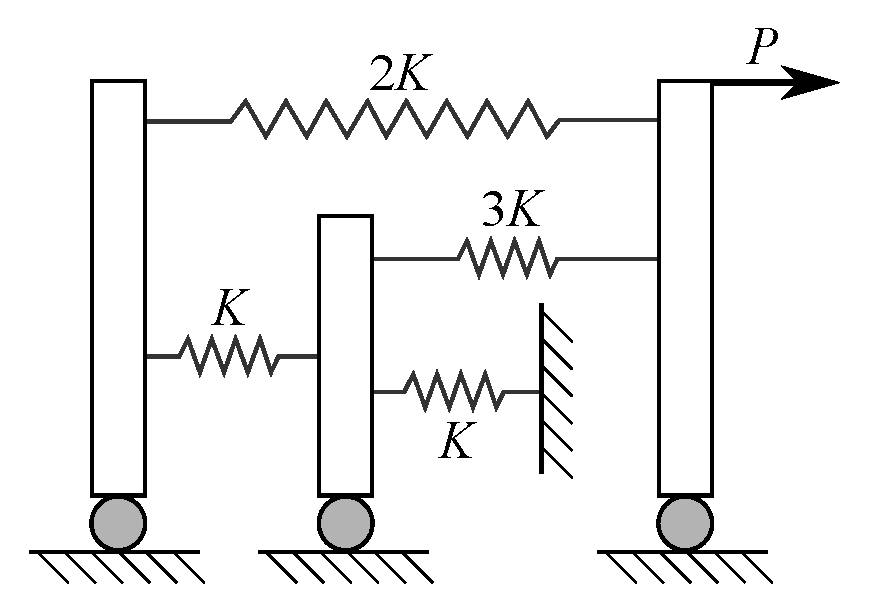
\includegraphics[width=10cm]{spring_system.pdf}
\caption{Typical assemblage of springs and masses.}
\label{fig:bathe}
\end{figure}


Consider a typical spring (finite element) like the one shown in \cref{fig:springel}
\begin{figure}[h]
\centering
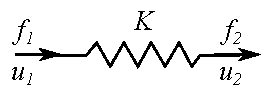
\includegraphics[width=8cm]{springel.pdf}
\caption{Typical spring element.}
\label{fig:springel}
\end{figure}

The relation between the force and the relative displacement can be written like
\[f_1 = K(u_1 - u_2)\]
and from equilibrium we have
\[f_1 + f_2 = 0\]
which yields the following force-displacement relationship for a typical spring element:
\begin{equation}
    \begin{Bmatrix}
        f_1\\
        f_2
    \end{Bmatrix} =
    K\begin{bmatrix}
          1.0 & -1.0\\
        - 1.0 & 1.0
    \end{bmatrix}
    \begin{Bmatrix}
        u_1\\
        u_2
    \end{Bmatrix}
    \label{eq:Kspring}
\end{equation}

On the other hand, the equilibrium equation for a typical mass with displacement $u_j$  (see \cref{fig:dclmass}) and attached to springs $i$ and $i+1$ reads
\begin{equation}
f_2^i + f_1^{i + 1} + m_j \dv{V_j}{t} = P_j.
\label{eq:equilmass}
\end{equation}
which can be written in terms of displacements using \cref{eq:Kspring} like
\[(K^i + K^{i + 1}) u_j - K^i u_{j - 1} - K^{i + 1} u_{j + 1} + m_j\dv{V_j}{t} = P_j .\]


\begin{figure}[H]
\centering
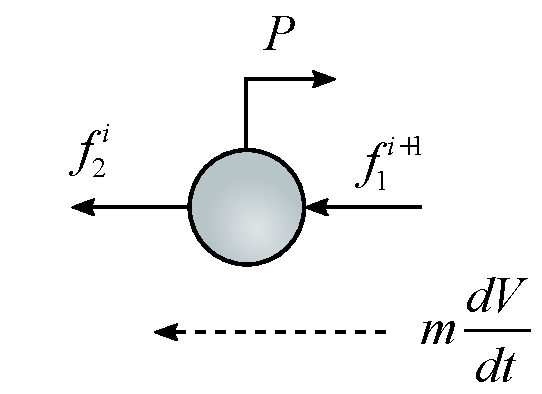
\includegraphics[width=8cm]{dcl_mass.pdf}
\caption{Free body diagram for a typical mass connected to springs $i$ and $i+1$.}
\label{fig:dclmass}
\end{figure}


Writing the elemental equilibrium equations in terms of $u_{j - 1}$, $u_j$ and $u_{j + 1}$ we have:

\[\left\{ {\begin{array}{*{20}{c}}
{f_1^i}\\
{f_2^i}
\end{array}} \right\} = \left[ {\begin{array}{*{20}{c}}
{k_{11}^i}&{k_{12}^i}\\
{k_{21}^i}&{k_{22}^i}
\end{array}} \right]\left\{ {\begin{array}{*{20}{c}}
{{u_{j - 1}}}\\
{{u_j}}
\end{array}} \right\}\]

and

\[\left\{ {\begin{array}{*{20}{c}}
{f_1^{i + 1}}\\
{f_2^{i + 1}}
\end{array}} \right\} = \left[ {\begin{array}{*{20}{c}}
{k_{11}^{i + 1}}&{k_{12}^{i + 1}}\\
{k_{21}^{i + 1}}&{k_{22}^{i + 1}}
\end{array}} \right]\left\{ {\begin{array}{*{20}{c}}
{{u_j}}\\
{{u_{j + 1}}}
\end{array}} \right\}\]

which gives for the equilibrium equation of the $m_j$ mass:

\[k_{21}^i{u_{j - 1}} + (k_{22}^i + k_{11}^{i + 1}){u_j} + k_{12}^{i + 1}{u_{j + 1}} + {m_j}\frac{{d{V_j}}}{{dt}} = {P_j}.\]

Considering also the contributions from the springs $K^i$ and $K^{i+1}$ to the equilibrium of masses $m_{j-1}$ and $m_{j+1}$ respectively we have the following matrix block:



\[\left[ {\begin{array}{*{20}{c}}
{}&{}&{}&{}\\
{}&{k_{11}^i}&{k_{12}^i}&{}\\
{}&{k_{21}^i}&{k_{22}^i + k_{11}^{i + 1}}&{k_{12}^{i + 1}}\\
{}&{}&{k_{21}^{i + 1}}&{k_{22}^{i + 1}}
\end{array}} \right]\]


Considering now the complete system of masses and springs leads to a system of linear equations of the form
\begin{equation}
\left[ {{K_G}} \right]\left\{ {{U_G}} \right\} + \left[ M \right]\left\{ {{A_G}} \right\} = \left\{ {{F_G}} \right\}.
\label{eq:global}
\end{equation}
where each equation represents the equilibrium of a given mass. The coefficient matrix in \cref{eq:global} can be assembled in a systematic way by establishing the connection between the global and local degrees of freedom. This can be accomplished through an operator storing in each row the global degrees of freedom corresponding to each element. For instance, \cref{fig:IBC} shows elements $K^i$ and $K^{i+1}$ and the global degrees of freedom corresponding to masses $m_{j-1}$, $m_j$ and $m_{j+1}$. The corresponding entries of the $DME$ operator for these elements are given by:


\[DME = \left[ {\begin{array}{*{20}{c}}
{}&{}\\
{j - 1}&j\\
j&{j + 1}\\
{}&{}
\end{array}} \right]\]

\begin{figure}[H]
\centering
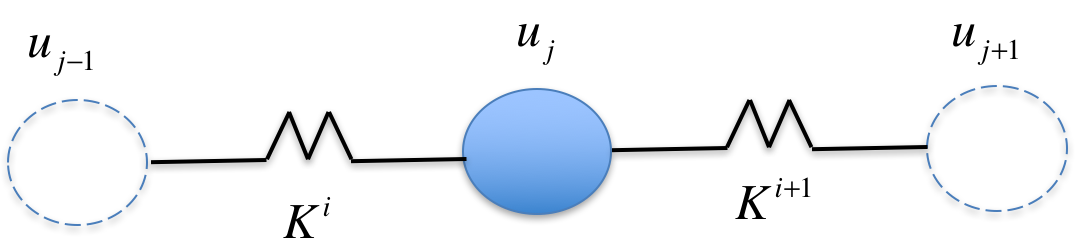
\includegraphics[width=12cm]{ibc}
\caption{Global degrees of freedom connected to the spring elements $K^i$ and $K^{i+1}$ respectively.}
\label{fig:IBC}
\end{figure}

and the contribution from these elements to the global coefficient matrix for elements $i$ and $i+1$ reads respectively:


\[\begin{array}{l}
{K_{j - 1,j - 1}} \leftarrow {K_{j - 1,j - 1}} + k_{11}^i\\
{K_{j - 1,j}} \leftarrow {K_{j - 1,j}} + k_{12}^i\\
{K_{j,j - 1}} \leftarrow {K_{j,j - 1}} + k_{21}^i\\
{K_{j,j}} \leftarrow {K_{j,j}} + k_{22}^i
\end{array}\]

and

\[\begin{array}{l}
{K_{j,j}} \leftarrow {K_{j,j}} + k_{11}^{i + 1}\\
{K_{j,j + 1}} \leftarrow {K_{j,j + 1}} + k_{12}^{i + 1}\\
{K_{j + 1,j}} \leftarrow {K_{j + 1,j}} + k_{21}^{i + 1}\\
{K_{j + 1,j + 1}} \leftarrow {K_{j + 1,j + 1}} + k_{22}^{i + 1}
\end{array}\]

The system given by \cref{eq:global}, assembled with the aid of the $DME$ operator can be solved for the global displacements $U_G$. The pseudo-code shown in \cref{algo:springs} presents all the steps required to solve the problem in the context of the finite element method. In that code the so-called DME operator is an equation assembly array indicating how each element contributes to the global stiffness and mass matrix.

\begin{algorithm}[H]\label{algo:springs}
    \SetAlgoLined
    \KwData{Problem parameters; NUMNP, NUMEL, NMATP}
    \KwResult{Displacements and spring forces}
    Create $DM$E operator\;
    Assemble $K^G$, $F^G$\;
    \While{$j \leq 1, NUMEL$}{
        $K^G \leftarrow K^G+K^i$\\
        $F^G \leftarrow F^G+F^i$\\
    }
    Solve $[K^G]U=F^G$\\
    Find internal forces
    \caption{Springs Algorithm.}    
\end{algorithm}

\newpage

\inputminted[]{python}{src/engine.py}

\newpage


\section{Basic elements of interpolation theory}
Let $f(x)$ be a function whose values are known at n discrete points ${x_1, x_2,...,x_n}$. We want to know (interpolate) the value of $f(x)$ at an arbitrary point $x \in \left[ {{x_1},{x_n}} \right]$.

\begin{figure}[h]
\centering
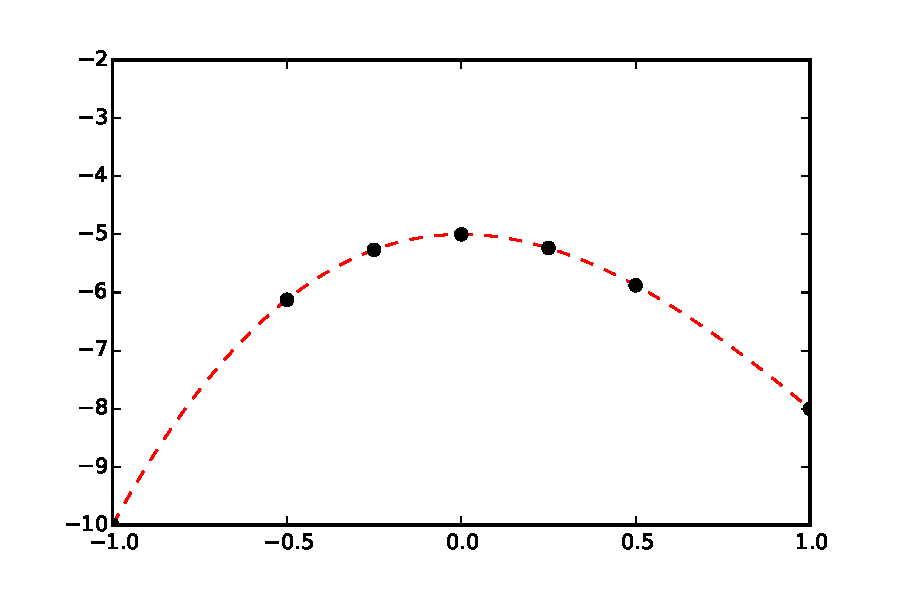
\includegraphics[width=12cm]{img/interpol1.pdf}
\caption{Global interpolation of a function}
\label{fig:interpol1}
\end{figure}

The process of interpolation or computation of the unknown value of $f(x)$ using the known values $\left\{ {{f^1},{f^2},...,{f^n}} \right\}$ involves two steps:

\begin{itemize}
\item[i]  Fitting an interpolating function to the known data points.
\item[ii] Evaluating the function at the arbitrary point.
\end{itemize}

We can (i) use all the n-data points and fit an $(n-1)$-th order polynomial (which is cumbersome and difficult to code) or (ii) split the domain in sub-intervals and use local polynomials within each sub-interval. This last approach involves only a couple of polynomials and it is easy to code, however it may have some continuity issues.

In finite element analysis local interpolation is used in order to proceed systematically. Local interpolation uses a finite number of nearest-neighbors and generates interpolated values $f(x)$ that do not in general have continuous first or higher derivatives.

\begin{figure}[h]
\centering
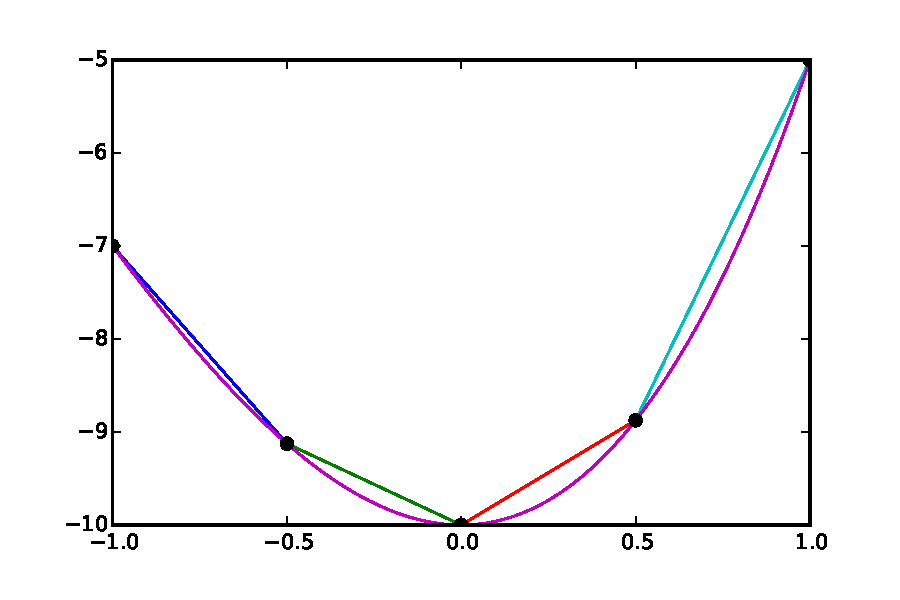
\includegraphics[width=12cm]{img/interpol2.pdf}
\caption{Local or piecewise interpolation of a function}
\label{fig:interpol2}
\end{figure}

\subsubsection{Lagrange interpolation theorem}
Given a set of n-points $\{ (x^1, y^1),\cdots,(x^n, y^n)\}$ where $y^n \equiv f({x^n})$ then: ``there exists a unique polynomial $p(x)$ of order at most $(n-1)$ such $p(x^I) = f(x^I)$ for $I=1,2,\cdots,n$". The polynomial is given by;
\begin{equation}\label{eq:pol}
  p(x^I) = L^I(x) f(x^I)  
\end{equation}
for $I=1,2,...,n$ where
\begin{equation}\label{eq:coef}
  L^I(x) = \prod_{\substack{J = 1\\ I \ne J}}^n \frac{(x - x^J)}{(x^I - x^J)}
\end{equation}
and where it should be noticed that
\[L^I(x^J) = \delta^{IJ}.\]

\subsubsection*{Example for n=3}
Consider the domain $[ - 1,1]$ and the data points at ${x^1} =  - 1.0$, ${x^2} =  + 1.0$ and ${x^3} = 0.0$. We have
\begin{align*}
& L^1(x) = \frac{(x - x^2)(x - x^3)}{(x^1 - x^2)(x^1-x^3)} \equiv  - \frac{1}{2}(1 - )x\\
& L^2(x) = \frac{(x - x^1)(x - x^3)}{(x^2 - x^1)(x^2 - x^3)} \equiv  + \frac{1}{2}(1 + x)x
\end{align*}
and
\[L^3(x) = \frac{(x - x^1)(x - x^2)}{(x^3 - x^1)(x^3 - x^2)} \equiv 1 - x^2.\]

The resulting interpolating polynomials $L^I(x)$ and the interpolating function  are shown in \cref{fig:pols} below
\begin{figure}[H]
  \centering
  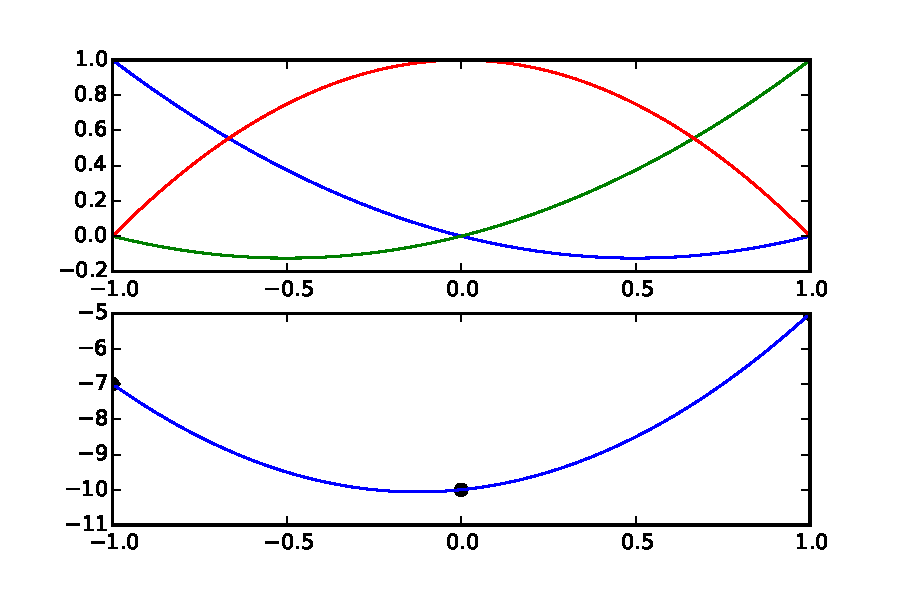
\includegraphics[width=16cm]{func.pdf}
  \caption{Interpolating polynomials and the resulting interpolating function}
  \label{fig:pols}
\end{figure}

\subsubsection*{Example: Interpolation of a function using a global and a local scheme}
Assume we have known values of the function:

\[f(x) = {x^3} + 4{x^2} - 10\]

in the interval $[-1.0, 1.0]$ and we wish to obtain an interpolated version of the function using different schemes.


\begin{figure}[H]
\centering
	\begin{subfigure}[b]{0.45\textwidth}\qquad
		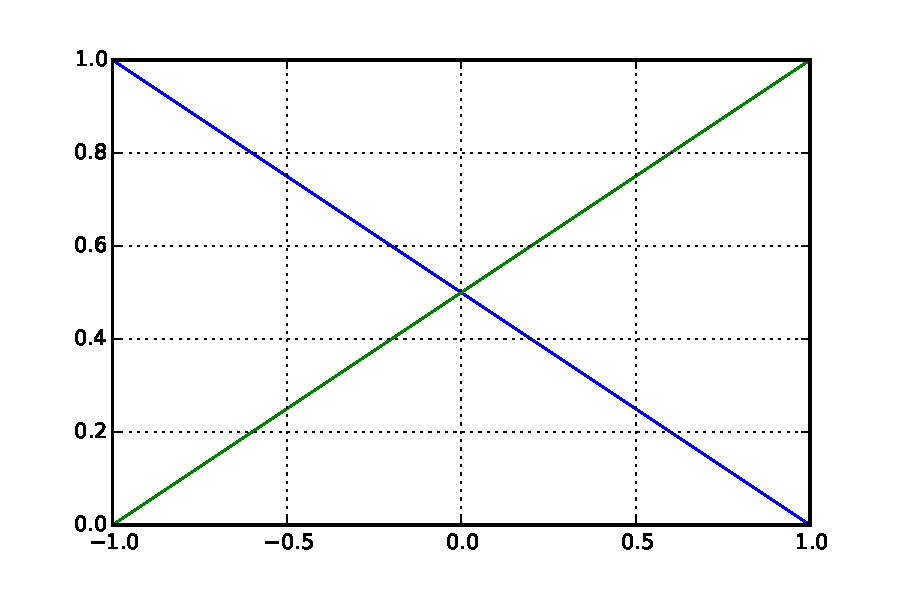
\includegraphics[width=\textwidth]{lineal.pdf}
		\caption{Interpolation polynomials. }
	\end{subfigure}\,
%
	\begin{subfigure}[b]{0.45\textwidth}\qquad
		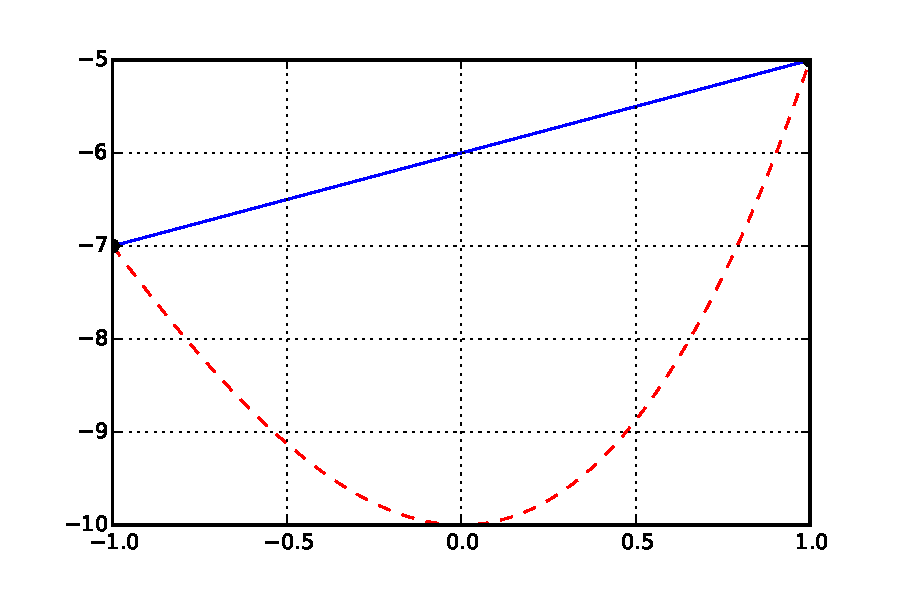
\includegraphics[width=\textwidth]{interlin.pdf}
		\caption{Actual and interpolated function.}
	\end{subfigure}\\
%
\centering
	\begin{subfigure}[b]{0.45\textwidth}\qquad
		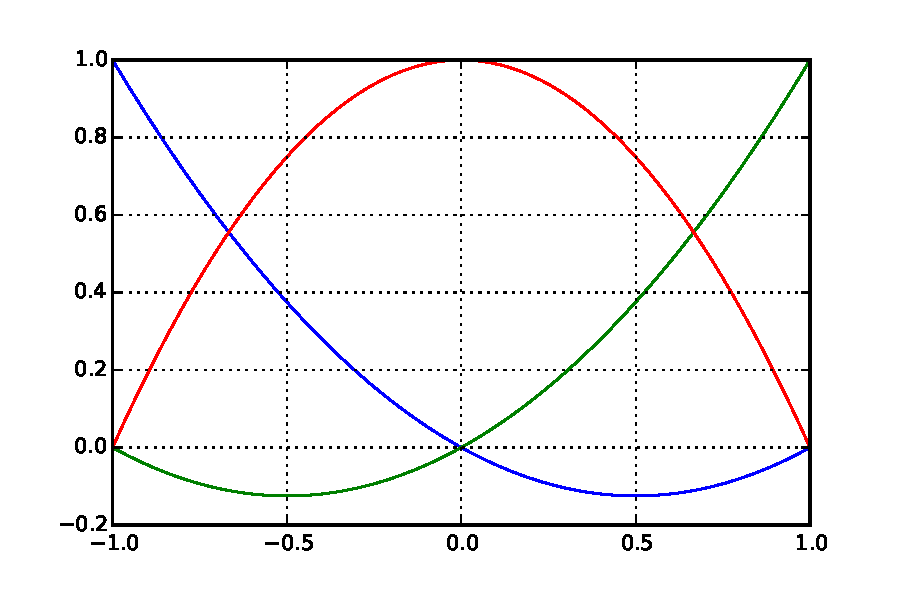
\includegraphics[width=\textwidth]{quadra.pdf}
		\caption{Interpolation polynomials.}
	\end{subfigure}\,
%
	\begin{subfigure}[b]{0.45\textwidth}\qquad
		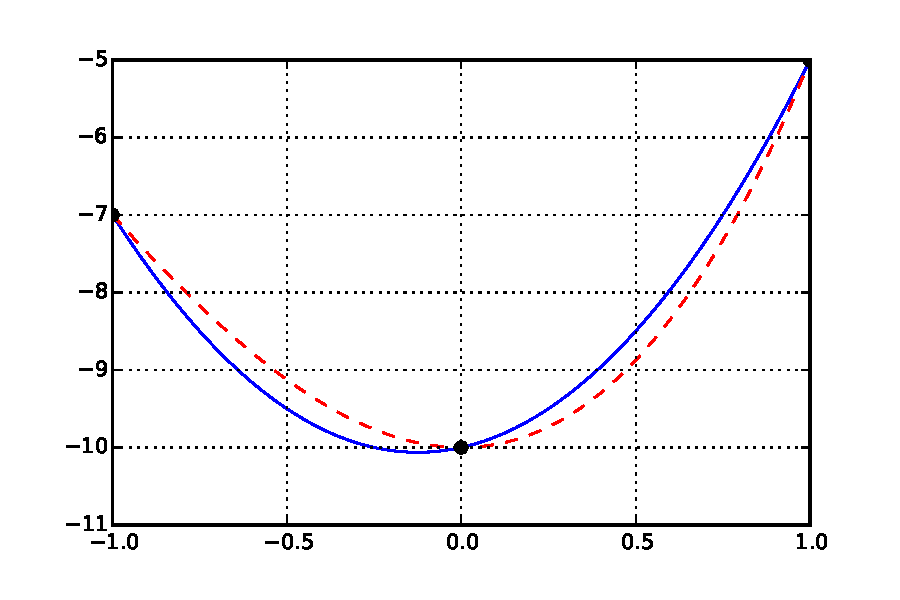
\includegraphics[width=\textwidth]{interqua.pdf}
		\caption{Actual and interpolated function.}
	\end{subfigure}\\
%
\centering
	\begin{subfigure}[b]{0.45\textwidth}\qquad
		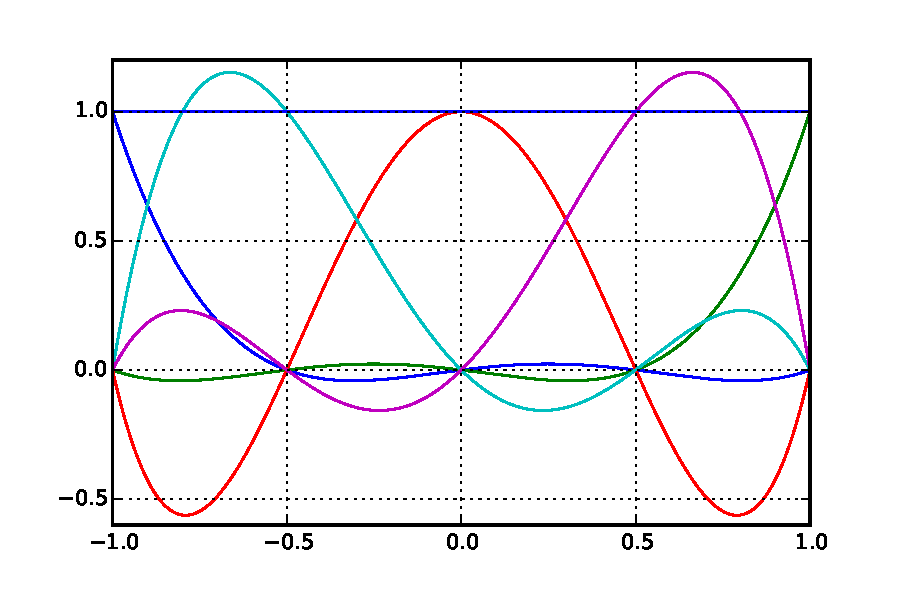
\includegraphics[width=\textwidth]{third.pdf}
		\caption{Interpolation polynomials.}
	\end{subfigure}\,
%
	\begin{subfigure}[b]{0.45\textwidth}\qquad
		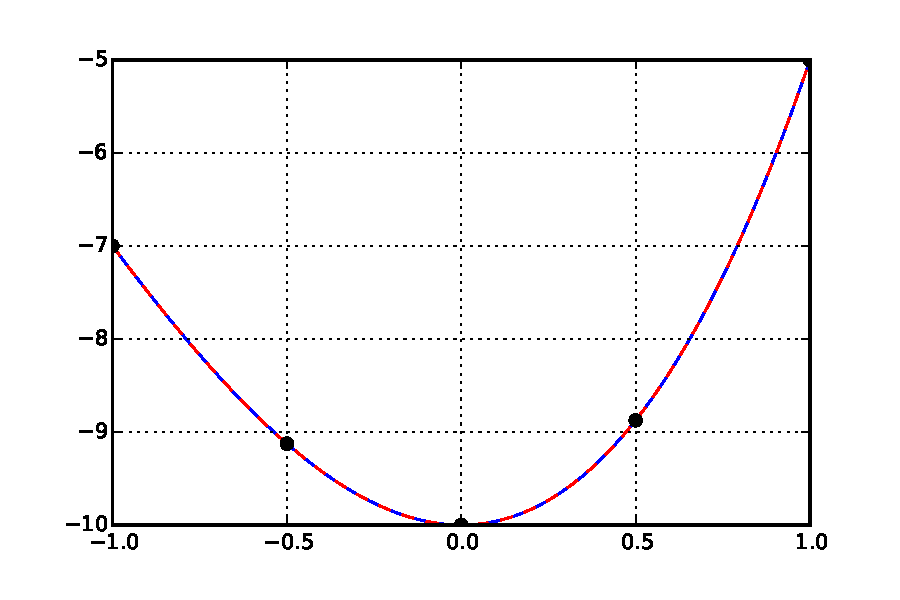
\includegraphics[width=\textwidth]{intertri.pdf}
		\caption{Actual and interpolated function.}
	\end{subfigure}
\caption{Lineal interpolation of the function $f(x) = {x^3} + 4{x^2} - 10$.}
\label{fig:several interpol}
\end{figure}

\Cref{fig:several interpol} shows the interpolating polynomials and the resulting function for the case of first, second and fourth order polynomials respectively. Similarly, the first order derivative obtained out of the interpolated function is displayed in \cref{fig:first der}. 

\begin{figure}[H]
\centering
	\begin{subfigure}[b]{0.45\textwidth}\qquad
		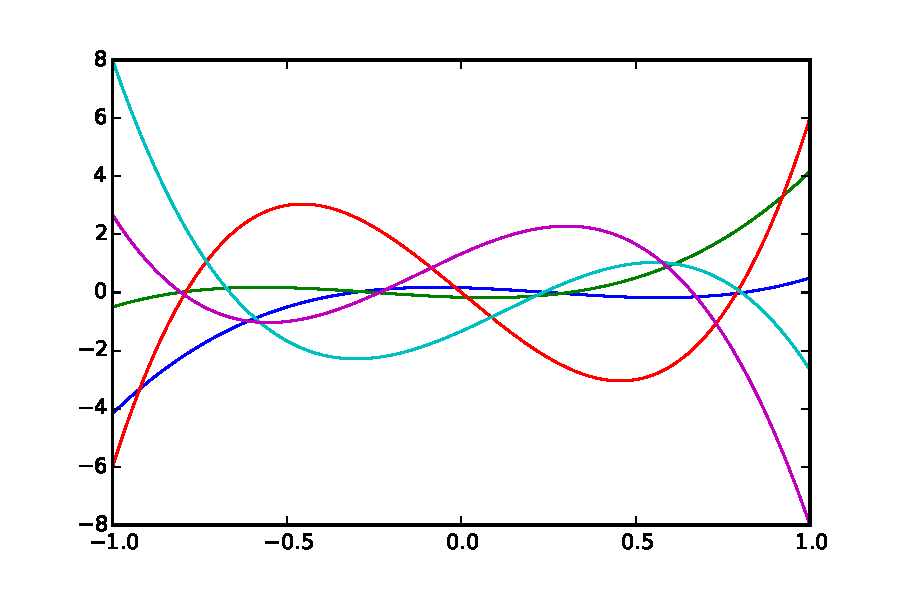
\includegraphics[width=\textwidth]{deriv2.pdf}
		\caption{First order derivatives of the interpolation polynomials. }
	\end{subfigure}\,
%
	\begin{subfigure}[b]{0.45\textwidth}\qquad
		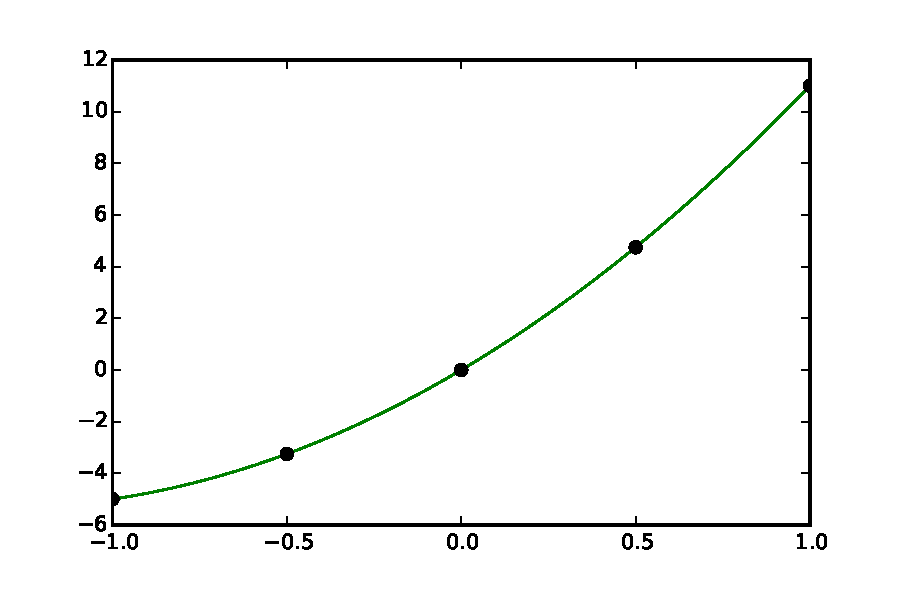
\includegraphics[width=\textwidth]{firstder.pdf}
		\caption{Interpolated first order derivative of the function.}
	\end{subfigure}\\

\caption{Lineal interpolation of the function $f(x) = {x^3} + 4{x^2} - 10$.}
\label{fig:first der}
\end{figure}

We now proceed like in the finite element method and use the local first order polynomials shown in \cref{fig:loc-pols} to interpolate the function under study.

\begin{figure}[H]
  \centering
  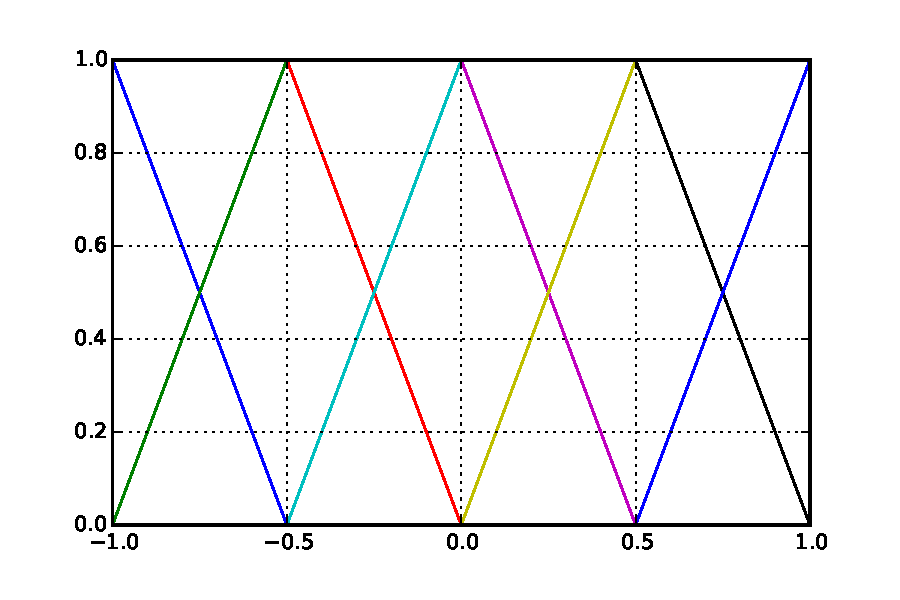
\includegraphics[width=10cm]{localone.pdf}
  \caption{Local interpolating polynomials}
  \label{fig:loc-pols}
\end{figure}

The resulting function and its numerically obtained first order derivateive are shown in \cref{fig:fully local}. It is clear how the local interpolation destroys the global continuity in the first order derivative while the function itself remains continous.


\begin{figure}[H]
\centering
	\begin{subfigure}[b]{0.45\textwidth}\qquad
		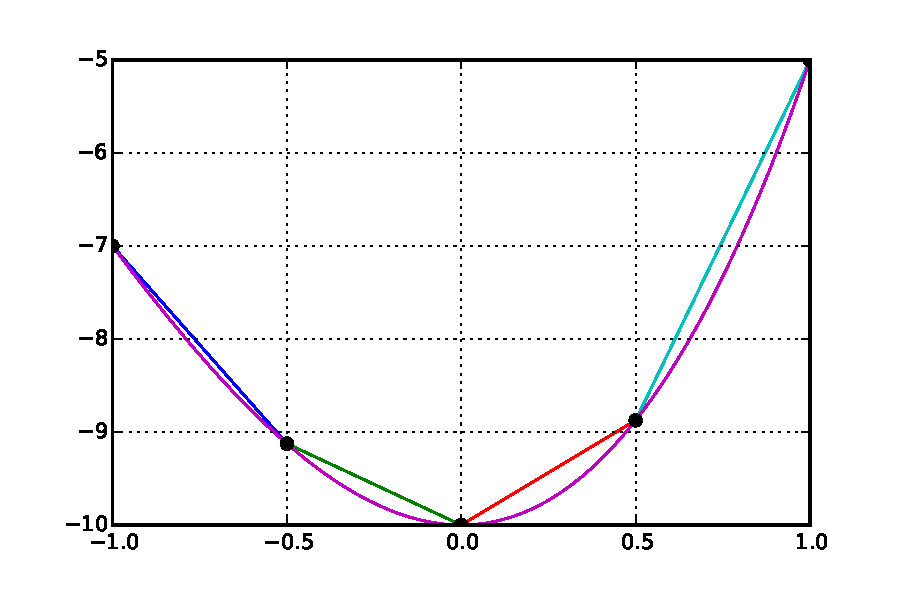
\includegraphics[width=\textwidth]{localfun.pdf}
		\caption{Function interpolated with local first order polynomials. }
	\end{subfigure}\,
%
	\begin{subfigure}[b]{0.45\textwidth}\qquad
		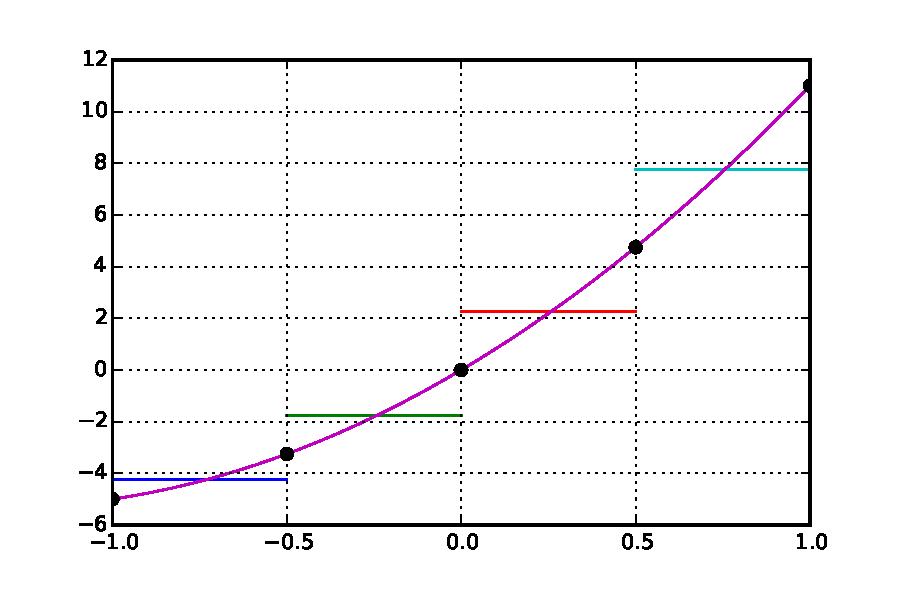
\includegraphics[width=\textwidth]{localfirst.pdf}
		\caption{Interpolated first order derivative of the function.}
	\end{subfigure}\\

\caption{Lineal interpolation of the function $f(x) = {x^3} + 4{x^2} - 10$.}
\label{fig:fully local}
\end{figure}

\subsection*{Extension to 2D domains}
Assume we are now interested in conducting interpolation of a function over a spatial 2-dimensional domain where every point is specified by a position vector of the form $\vb{x} = x \hat{\imath} + y\hat{\jmath}$. We want to know, via interpolation, the value of a function $f(\vb{x})$ at an arbitrary point $\vb{x}$ provided we know the set of n-points $\{(\vb{x}^1, f^1),\cdots,(\vb{x}^n, f^n)\}$.
\begin{figure}[H]\label{fig:element}
  \centering
  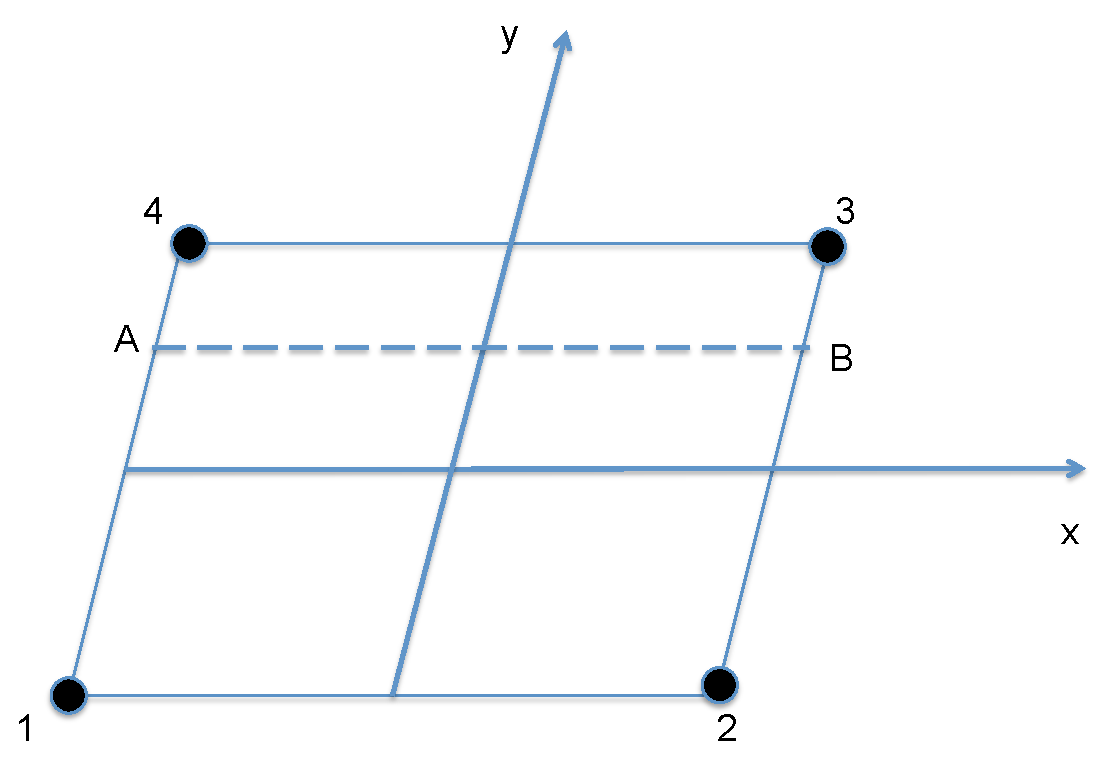
\includegraphics[width=10cm]{element.pdf}
  \caption{Basic square domain}
\end{figure}

We first fix $x = x^A$ and conduct 1-dimensional interpolation along the $y$ direction as discussed in the previous section as follows (see \cref{fig:onedimn})
\[f(x^A,y) = L^1(y)f^1 + L^4(y)f^4\]

\begin{figure}[H]
\centering
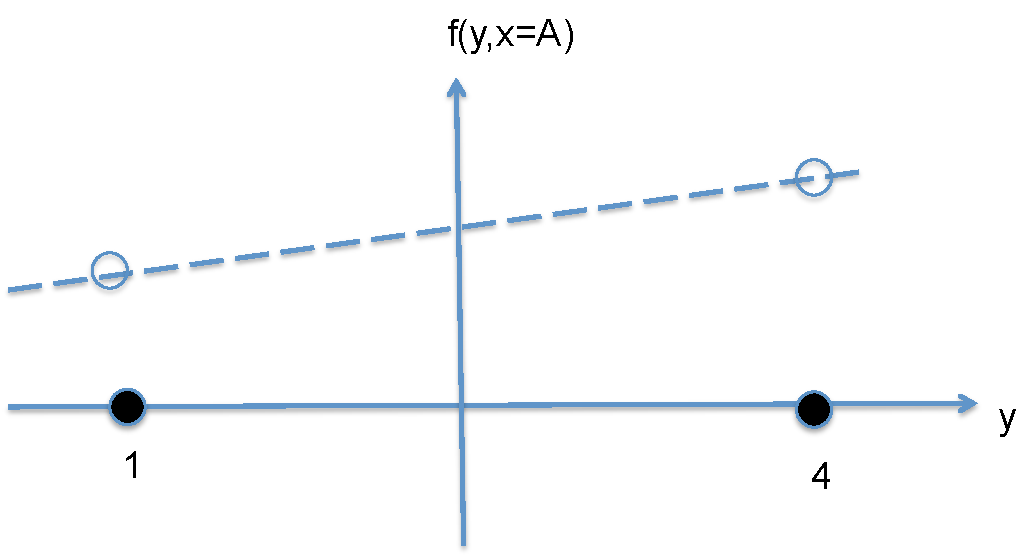
\includegraphics[width=10cm]{inter1D.pdf}
\caption{Interpolation along the $y$-direction}
\label{fig:onedimn}
\end{figure}

Similarly, we can fix $x = x^B$ and interpolate once again along the $y$ direction
\[f(x^B,y) = L^2(y)f^2 + L^3(y)f^3.\]

We now conduct the interpolation along the $x$-direction using the functions $f(x^A,y)$ and $f(x^B,y)$ respectively as follows
\begin{align*}
  &f(x,y) = L^A(x) f(x^A,y) + L^B(x)f(x^B,y)\\
  &f(x,y) = L^A(x)\{L^1(y)f^1 + L^4(y)f^4\} + L^B(x)\{L^2(y)f^2 + L^3(y)f^3\}\\
  &f(x,y) = L^A(x)L^1(y)f^1 + L^A(x)L^4(y)f^4 + L^B(x)L^2(y)f^2 + L^B(x)L^3(y)f^3 \enspace ,
\end{align*}
where
\begin{align*}
L^A(x) & \equiv L^1(x)\\
L^B(x) & \equiv L^2(x)\\
L^1(y) & \equiv L^1(y)\\
L^2(y) & \equiv L^1(y)\\
L^3(y) & \equiv L^2(y)\\
L^4(y) & \equiv L^2(x) \enspace .
\end{align*}

The function of two variables is then written as the product of one-dimensional interpolations
\[f(x,y) = N^1(x,y)f^1 + N^2(x,y)f^2 + N^3(x,y)f^3 + N^4(x,y)f^4\]
with
\begin{align*}
N^1(x,y) & = L^1(x)L^1(y)\\
N^2(x,y) & = L^2(x)L^1(y)\\
N^3(x,y) & = L^2(x)L^2(y)\\
N^4(x,y) & = L^1(x)L^2(y) \enspace .
\end{align*}

See Figure \ref{fig:four-nodes-interp} for the shape functions of a 4-nodes element.
\begin{figure}[H]
\centering
	\begin{subfigure}[b]{0.45\textwidth}\qquad
		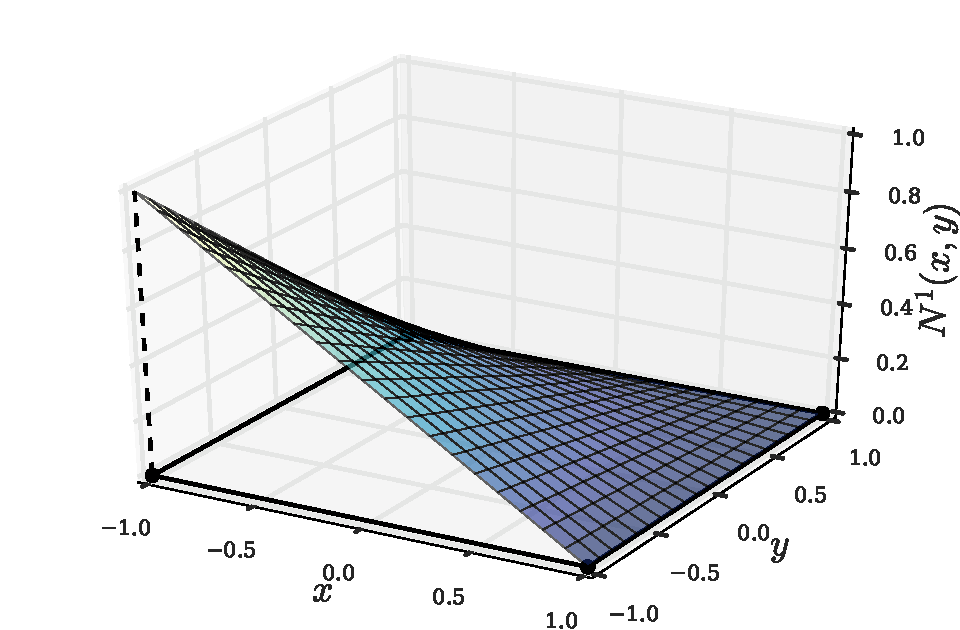
\includegraphics[width=\textwidth]{shape_func-4-nodes-1.pdf}
		\caption{Shape function ${N^1(x,y)=\frac{1}{4}(1-x)(1-y)}$. }
	\end{subfigure}\,
%
	\begin{subfigure}[b]{0.45\textwidth}\qquad
		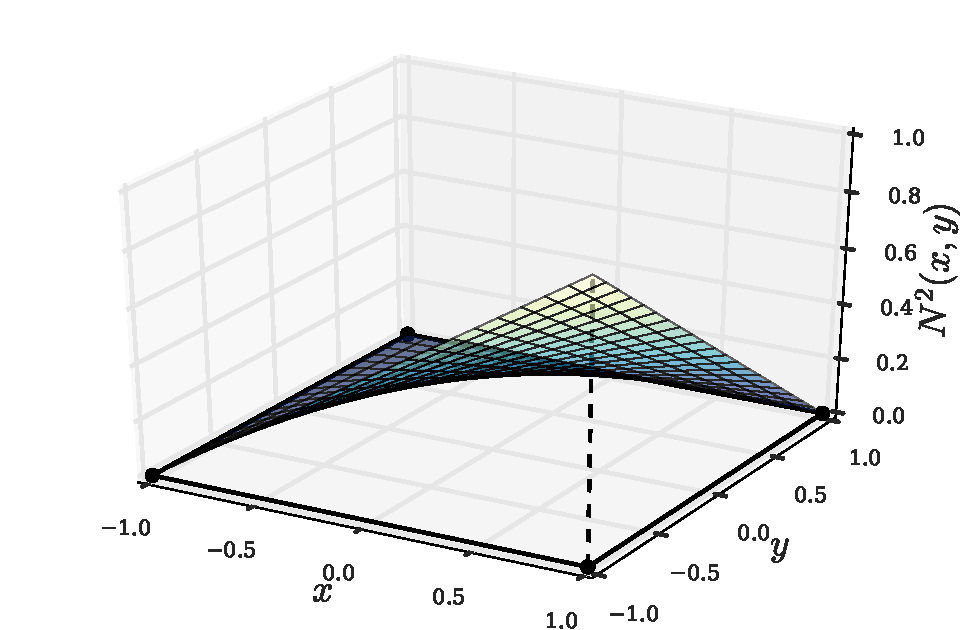
\includegraphics[width=\textwidth]{shape_func-4-nodes-2.pdf}
		\caption{Shape function ${N^2(x,y)=\frac{1}{4}(1+x)(1-y)}$.}
	\end{subfigure}\\
%
	\begin{subfigure}[b]{0.45\textwidth}\qquad
		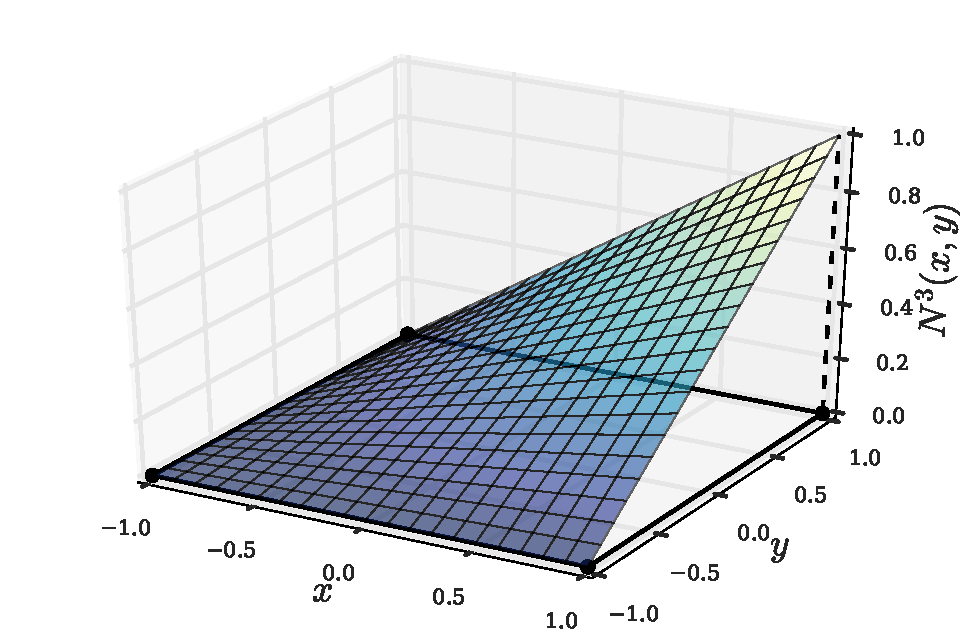
\includegraphics[width=\textwidth]{shape_func-4-nodes-3.pdf}
		\caption{Shape function ${N^3(x,y)=\frac{1}{4}(1+x)(1+y)}$.}
	\end{subfigure}\,
%
	\begin{subfigure}[b]{0.45\textwidth}\qquad
		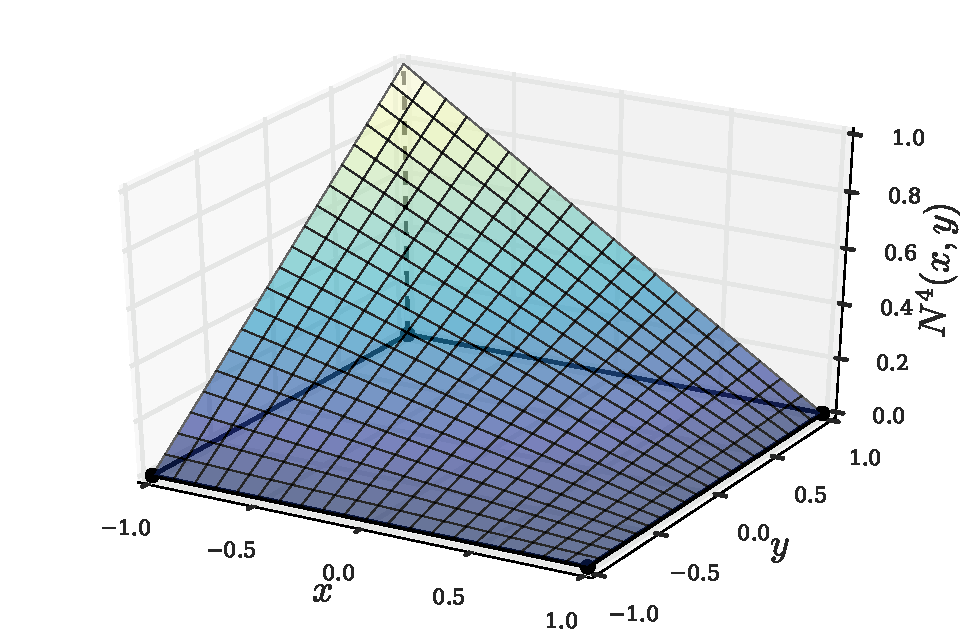
\includegraphics[width=\textwidth]{shape_func-4-nodes-4.pdf}
		\caption{Shape function ${N^4(x,y)=\frac{1}{4}(1-x)(1+y)}$.}
	\end{subfigure}
\caption{Shape functions for a 4-nodes element.}
\label{fig:four-nodes-interp}
\end{figure}

See Figure \ref{fig:nine-nodes-interp} for the shape functions of a 9-nodes element.
\begin{figure}[H]
\centering
	\begin{subfigure}[b]{0.45\textwidth}\qquad
		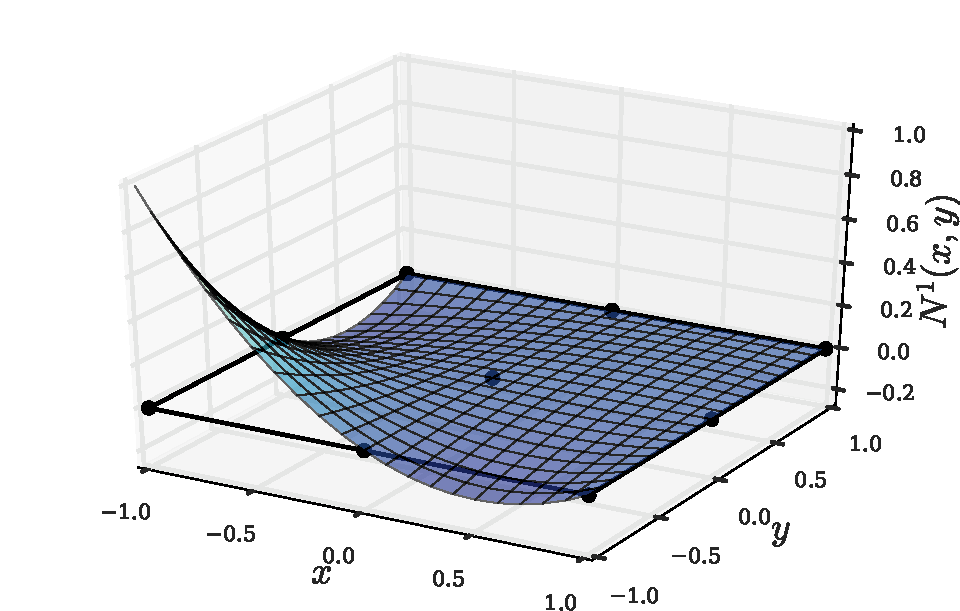
\includegraphics[width=\textwidth]{shape_func-9-nodes-1.pdf}
		\caption{Shape function $N^1(x,y)$. }
	\end{subfigure}\,
%
	\begin{subfigure}[b]{0.45\textwidth}\qquad
		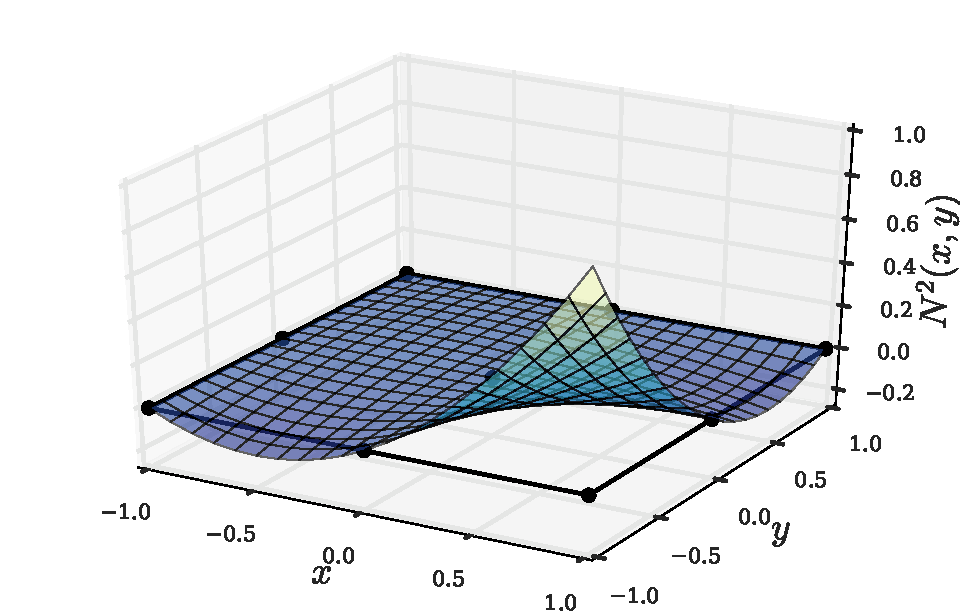
\includegraphics[width=\textwidth]{shape_func-9-nodes-2.pdf}
		\caption{Shape function $N^2(x,y)$.}
	\end{subfigure}\\
%
	\begin{subfigure}[b]{0.45\textwidth}\qquad
		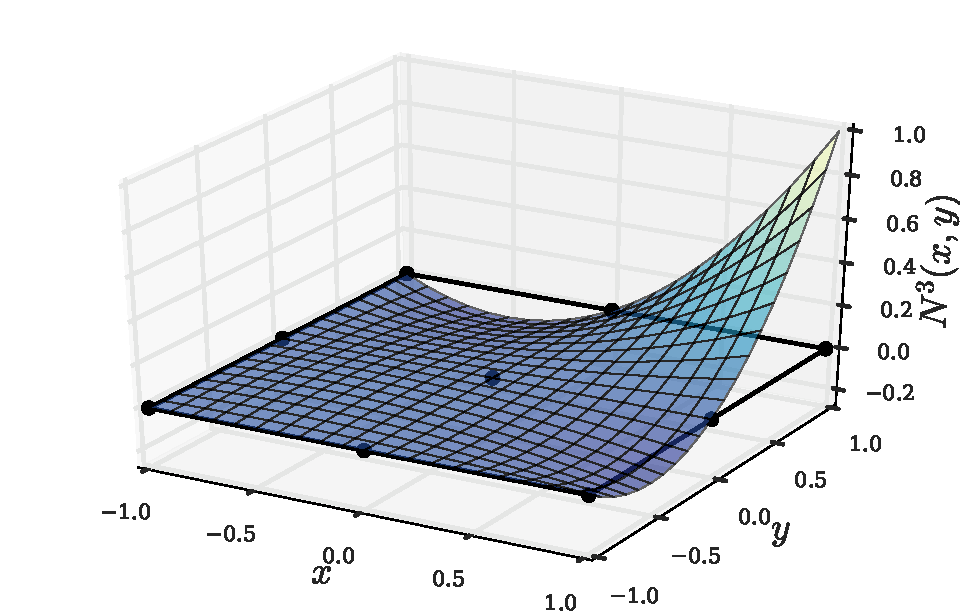
\includegraphics[width=\textwidth]{shape_func-9-nodes-3.pdf}
		\caption{Shape function $N^3(x,y)$.}
	\end{subfigure}\,
%
	\begin{subfigure}[b]{0.45\textwidth}\qquad
		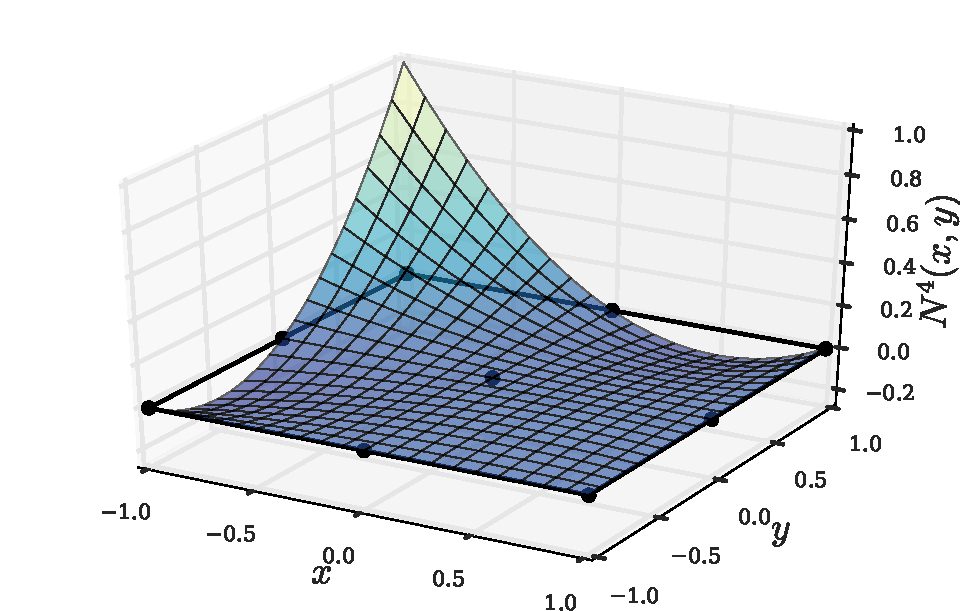
\includegraphics[width=\textwidth]{shape_func-9-nodes-4.pdf}
		\caption{Shape function $N^4(x,y)$.}
	\end{subfigure}\\
	%
	\begin{subfigure}[b]{0.45\textwidth}\qquad
		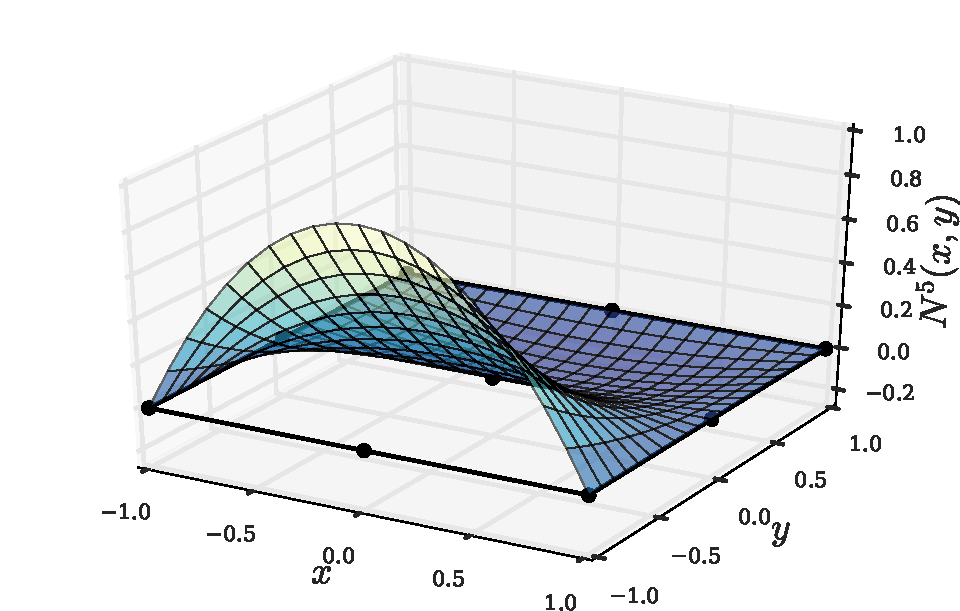
\includegraphics[width=\textwidth]{shape_func-9-nodes-5.pdf}
		\caption{Shape function $N^5(x,y)$.}
	\end{subfigure}\,
%
	\begin{subfigure}[b]{0.45\textwidth}\qquad
		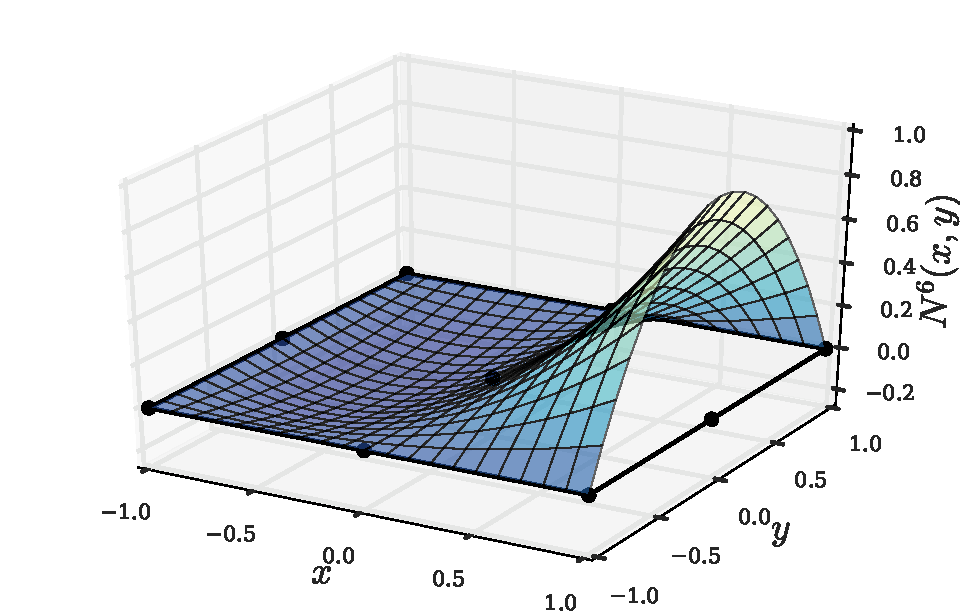
\includegraphics[width=\textwidth]{shape_func-9-nodes-6.pdf}
		\caption{Shape function $N^6(x,y)$.}
	\end{subfigure}
	\caption{Shape functions for a 9-nodes element.}
	\label{fig:nine-nodes-interp}
\end{figure}
%
\begin{figure} [H]
	\ContinuedFloat
	\centering
	\begin{subfigure}[b]{0.45\textwidth}\qquad
		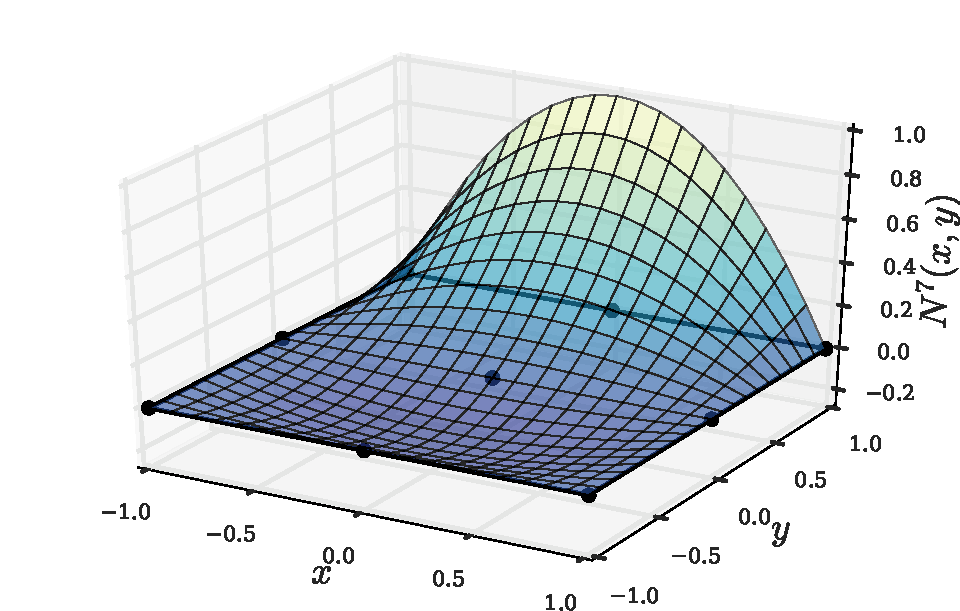
\includegraphics[width=\textwidth]{shape_func-9-nodes-7.pdf}
		\caption{Shape function $N^7(x,y)$.}
	\end{subfigure}\,
%
	\begin{subfigure}[b]{0.45\textwidth}\qquad
		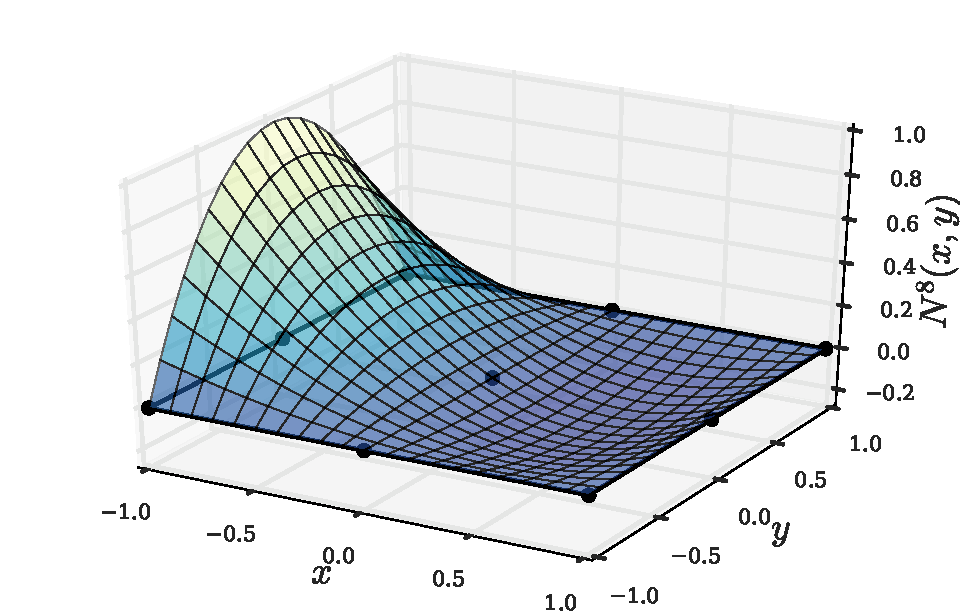
\includegraphics[width=\textwidth]{shape_func-9-nodes-8.pdf}
		\caption{Shape function $N^8(x,y)$.}
	\end{subfigure}\\
	%
	\begin{subfigure}[b]{0.45\textwidth}\qquad
		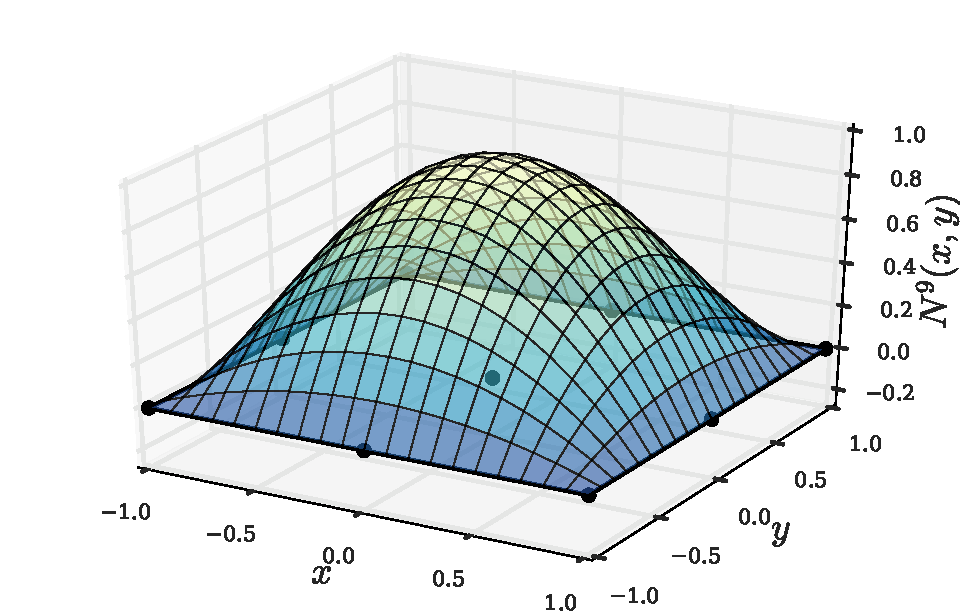
\includegraphics[width=\textwidth]{shape_func-9-nodes-9.pdf}
		\caption{Shape function $N^9(x,y)$.}
	\end{subfigure}
\caption{Shape functions for a 9-nodes element. (Continued)}
\end{figure}

\section[Discretization of the PVW using FEM]{Discretization of the PVW via the FEM}
\subsection{Formulation of the finite element matrices}
We now discretize the principle of virtual work repeated below for completeness:
\begin{equation} \label{pvw_2}
\intL_V \sigma_{ij} \delta u_{i,j} \dd{V} - \intL_V f_i \delta u_i \dd{V} - \intL_{S_t} t_i^n \delta u_i \dd{S} = 0.
\end{equation}

For that purpose we will divide the complete domain $V$ into $N$-finite non-overlapping sub-domains over each one of which we will approximate the solution in terms of local interpolating functions (see \cref{fig:fully local}). Since the PVW (or weak form of the BVP) has been cast into an integral representation, it is possible to build the total integral considering the contribution of the $N$-sub-domains like:
\begin{equation}\label{pvw_dis}
\sum_{e=1}^{NEL} \intL_{V^e} \sigma_{ij} \var{u}_{i,j} \dd{V^e} - \intL_V f_i \var{u}_i \dd{V^e} - \intL_{S_t} t_i^n \var{u}_i\dd{S^e} = 0 
\end{equation}

For simplicity we consider only a single element or sub-domain, thus;

\begin{equation}\label{pvw_sing}
\intL_V \sigma_{ij} \delta\epsilon_{i,j} dV - \intL_V f_i\delta u_idV - \intL_{S_t} t_i^n \delta u_i dS = 0
\end{equation}

where it is assumed that the discretized version of each element is later added up (or assembled) into the global equations for the complete model and where we have already used the fact that $\sigma_{ij}$ is symmetric impliying that $\sigma_{ij} \delta u_{i,j} = \sigma_{ij} \delta\epsilon_{i,j}$.

The involved functions (e.g., displacements, strain, stresses) will be approximated via interpolation of the solution over a determined number of points termed in what follows nodes. Assume for instance that over element $e$ containing $n$ such nodes we know the displacements vector $u_i$. For instance, \cref{fig:simple element} below shows a typical square 4-noded element of side $2h$. The rectangular components of the displacement vector at each node are labeled like $[u_1, u_2,...,u_7, u_8]$.

\begin{figure}[H]
\centering
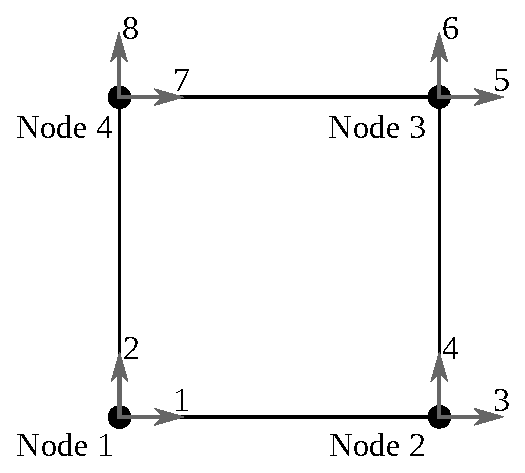
\includegraphics[width=7cm]{lado2h.pdf}
\caption{Square element of side $2h$.}
\label{fig:simple element}
\end{figure}


Furthermore, in a more general treatment, we let the displacements for an arbitrary $p$-node of a $3D$ problem $u^P=[u^P, v^P, w^P]$. Using ideas from interpolation theory it is now possible to approximate the displacements vector over an arbitrary point $\vb{x}$ inside the element by;

\[u_i(\vb x) = N_i^1(\vb x)u^1 + N_i^2(\vb x)u^2 + \cdots + N_i^P(\vb x)u^P + \cdots + N_i^n(\vb x)u^n\]

or in more general form

\begin{equation} \label{bas_interpol}
{u_i}(\vb x) = N_i^Q(\vb x){u^Q}
\end{equation}

and where the caption superscripts indicate summation over the number of nodes of the element while the subscript refers to the physical character of the variable being interpolated.

Now let us use the kinematic relationshio between strains and displpacements:

\[ \varepsilon_{ij}(\vb x) = \frac{1}{2}( u_{i,j} + u_{j,i} ) \]

together with \cref{bas_interpol}. Carrying the derivatives into the shape functions yields;

\[ \varepsilon_{ij}(\vb x) = \frac{1}{2}\left(\pdv{N_i^Q}{x_j} + \pdv{N_j^Q}{x_i} \right){u^Q} \]

which can be written like

\begin{equation}
\varepsilon_{ij}(\vb x) = B_{ij}^Q(\vb x){u^Q}
\label{str-dis}
\end{equation}

after letting

\[ B_{ij}^Q = \frac{1}{2}\left(\pdv{N_i^Q}{x_j} + \pdv{N_j^Q}{x_i} \right). \]

Proceeding analogously for the virtual fields after using
\[ \delta {u_i} = N_i^Q(\vb x)\delta {u^Q} \]
gives us:
\[ \intL_V C_{ijkl} B_{kl}^P u^P B_{ij}^Q\delta u^Q \dd{V} - \intL_V f_i N_i^Q\delta {u^Q}\dd{V}  - \intL_{S_t} t_i^n N_i^Q\delta {u^Q} \dd{S} = 0 \]
which can be re-organized into
\[ \delta {u^Q}\intL_V B_{ij}^Q C_{ijkl} B_{kl}^P\dd{V}{u^P} - \delta {u^Q}\intL_V N_i^Q{f_i}\dd{V}  - \delta {u^Q}\intL_{S_t} N_i^Qt_i^n\dd{S} = 0\]
which is the generalized discrete version of the PVW for a single element consistent with \cref{pvw_sing}. Defining the terms corresponding to the integrals like:
\begin{equation}
\begin{aligned}
{K^{QP}} & = \int\limits_V {{C_{ijkl}}B_{kl}^PB_{ij}^QdV} \\
f_c^Q    & = \int\limits_S {N_i^Qt_i^ndS} \\
f_V^Q    & = \int\limits_V {N_i^Q{f_i}dV}
\label{Rigi_3}
\end{aligned}
\end{equation}


allows us to write:


\[ \delta u^Q f_\sigma ^Q - \delta {u^Q}f_V^Q - \delta u^Q f_c^Q = 0. \]

This equation is once again the generalized discrete version of the PVW corresponding to the $Q$-displacement degree of freedom. The equation quantifies the work of the forces along the $Q$-th degree of freedom over the virtual displacements $\delta u^Q$. If we now use the arbitrary character of the virtual field $\delta u^Q $ we can write;

\begin{equation}
f_\sigma ^Q - f_V^Q - f_c^Q = 0.
\label{forces}
\end{equation}

This is now a mechanical equilibrium equation relating the forces along the $Q$-th degree of freedom associated to the internal element stresses $f_\sigma ^Q$; the external body forces $f_V^Q$ and the applied external tractions $f_c^Q$. Introducing the stiffness of the element gives:

\begin{equation}
K^{QP} u^P = f_V^Q + f_c^Q.
\label{Discreta}
\end{equation}

\subsubsection{Formulation of the stiffness matrix in perfectly square elements}
In the previous section we recognized:

\begin{equation}
\begin{aligned}
{K^{QP}} & = \int\limits_V {{C_{ijkl}}B_{kl}^PB_{ij}^QdV} \\
f_c^Q    & = \int\limits_S {N_i^Qt_i^ndS} \\
f_V^Q    & = \int\limits_V {N_i^Q{f_i}dV}
\label{Rigi}
\end{aligned}
\end{equation}



as the elemental stiffness matrix and the vectors of consistent contact and body forces for a single element. Let us assume that the domain of the single element is a perfect square of side $2h$ (see \cref{fig:lado2h}), thus;

\begin{equation}
\begin{aligned}
K & = \int\limits_{ - h}^{ + h} {\int\limits_{ - h}^{ + h} {{B^T}CBdxdy} } \\
{f_c} & = \int\limits_{ - h}^{ + h} {{N^T}{t^n}ds} \\
{f_v} & = \int\limits_{ - h}^{ + h} {\int\limits_{ - h}^{ + h} {{N^T}fdxdy} }
\label{ele2}
\end{aligned}
\end{equation}

\begin{figure}[H]
\centering
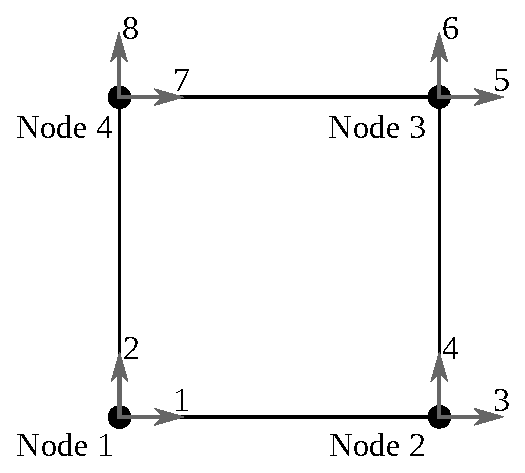
\includegraphics[width=7cm]{lado2h.pdf}
\caption{Square element of side $2h$.}
\label{fig:lado2h}
\end{figure}


and where $N$ and $B$ are the displacements interpolation matrix and the strain-displacements interpolation matrix respectively. For the linear 4-noded element shown in \cref{fig:lado2h} these matrices have the form defined in the following interpolation equations:


\[\left\{ {\begin{array}{*{20}{c}}
{u(\vec x)}\\
{v(\vec x)}
\end{array}} \right\} = \left[ {\begin{array}{*{20}{c}}
{{N^1}(\vec x)}&0&{{N^2}(\vec x)}&0&{{N^3}(\vec x)}&0&{{N^4}(\vec x)}&0\\
0&{{N^1}(\vec x)}&0&{{N^2}(\vec x)}&0&{{N^3}(\vec x)}&0&{{N^4}(\vec x)}
\end{array}} \right]\left\{ {\begin{array}{*{20}{c}}
{{u^1}}\\
{{u^2}}\\
{{u^3}}\\
{{u^4}}\\
{{u^5}}\\
{{u^6}}\\
{{u^7}}\\
{{u^8}}
\end{array}} \right\}\]


\[\left\{ {\begin{array}{*{20}{c}}
{\frac{{\partial u}}{{\partial x}}}\\
{\frac{{\partial v}}{{\partial y}}}\\
{\frac{{\partial v}}{{\partial x}} + \frac{{\partial u}}{{\partial y}}}
\end{array}} \right\} = \left[ {\begin{array}{*{20}{c}}
{\frac{{\partial {N^1}(\vec x)}}{{\partial x}}}&0&{\frac{{\partial {N^2}(\vec x)}}{{\partial x}}}&0&{\frac{{\partial {N^3}(\vec x)}}{{\partial x}}}&0&{\frac{{\partial {N^4}(\vec x)}}{{\partial x}}}&0\\
0&{\frac{{\partial {N^1}(\vec x)}}{{\partial y}}}&0&{\frac{{\partial {N^2}(\vec x)}}{{\partial y}}}&0&{\frac{{\partial {N^3}(\vec x)}}{{\partial x}}}&0&{\frac{{\partial {N^4}(\vec x)}}{{\partial x}}}\\
{\frac{{\partial {N^1}(\vec x)}}{{\partial x}}}&{\frac{{\partial {N^1}(\vec x)}}{{\partial y}}}&{\frac{{\partial {N^2}(\vec x)}}{{\partial x}}}&{\frac{{\partial {N^2}(\vec x)}}{{\partial y}}}&{\frac{{\partial {N^3}(\vec x)}}{{\partial x}}}&{\frac{{\partial {N^3}(\vec x)}}{{\partial y}}}&{\frac{{\partial {N^4}(\vec x)}}{{\partial x}}}&{\frac{{\partial {N^4}(\vec x)}}{{\partial y}}}
\end{array}} \right]\left\{ {\begin{array}{*{20}{c}}
{{u^1}}\\
{{u^2}}\\
{{u^3}}\\
{{u^4}}\\
{{u^5}}\\
{{u^6}}\\
{{u^7}}\\
{{u^8}}
\end{array}} \right\}\]

with the independent shape functions being:


\begin{align*}
{N^1}(x) & = \frac{1}{4}(1 - x)(1 - y) \\
{N^2}(x) & = \frac{1}{4}(1 + x)(1 - y) \\
{N^3}(x) & = \frac{1}{4}(1 + x)(1 + y) \\
{N^4}(x) & = \frac{1}{4}(1 - x)(1 + y)
\end{align*}




Notice that in the computation of the stiffness matrix we actually require the spatial derivatives of the shape functions given by;

\begin{align*}
\frac{{\partial {N^1}(x)}}{{\partial x}} & =  - \frac{1}{4}(1 - y)           &  \frac{{\partial {N^1}(x)}}{{\partial y}} & =  - \frac{1}{4}(1 - x)\\
\frac{{\partial {N^2}(x)}}{{\partial x}} & =  + \frac{1}{4}(1 - y)           &  \frac{{\partial {N^2}(x)}}{{\partial y}} & =  - \frac{1}{4}(1 + x)\\
\frac{{\partial {N^3}(x)}}{{\partial x}} & =  + \frac{1}{4}(1 + y)           &  \frac{{\partial {N^3}(x)}}{{\partial y}} & =  + \frac{1}{4}(1 + x)\\
\frac{{\partial {N^4}(x)}}{{\partial x}} & =  - \frac{1}{4}(1 + y)           &  \frac{{\partial {N^4}(x)}}{{\partial y}} & =  + \frac{1}{4}(1 - y)
\end{align*}


The contribution to the element matrix from a typical nodal point is thus given by;



\[K = \int\limits_{ - h}^{ + h} {\int\limits_{ - h}^{ + a} {\begin{bmatrix}

 \vdots &  \vdots & \vdots &  \vdots & \vdots & \vdots \\
 \cdots &  \frac{{\partial {N^K}(x)}}{{\partial x}} & 0   & \frac{{\partial {N^K}(x)}}{{\partial y}} &  \cdots & \cdots \\
  \cdots &  0 & \frac{{\partial {N^K}(x)}}{{\partial y}}   & \frac{{\partial {N^K}(x)}}{{\partial x}} &  \cdots & \cdots \\
 \vdots &  \vdots & \vdots &  \vdots & \vdots & \vdots 

\end{bmatrix}
%
\begin{bmatrix}
 A & B &  0\\
 B & A & 0 \\
 0 &  0 & C
\end{bmatrix}
%
\begin{bmatrix}
 \cdots & \frac{{\partial {N^Q}(x)}}{{\partial x}} & 0  & \cdots \\
 \cdots & 0 & \frac{{\partial {N^Q}(x)}}{{\partial y}}  & \cdots \\
 \cdots & \frac{{\partial {N^Q}(x)}}{{\partial y}} & \frac{{\partial {N^Q}(x)}}{{\partial x}}  & \cdots 
\end{bmatrix} dxdy} } \]


while a typical element of the resultant stiffness matrix takes the general form:
\[K \equiv A\int\limits_{- h}^{ + h} \int\limits_{-h}^{+h} \pdv{N^K}{x}\pdv{N^Q}{x}\dd{x}\dd{y}  + C\int\limits_{-h}^{+h} \int\limits_{-h}^{+h}\pdv{N^K}{y}\pdv{N^Q}{x}\dd{x}\dd{y}.\]
It should be noticed that for the considered perfectly square element the resulting stiffness matrix can be partitioned into factors which depend upon the material properties only and into a single factor which depends on the size $h$. This last contribution can be obtained analytically.

Once the elemental matrices are obtained these are assembled into the final global system of equations. Details of the assembly process are discussed in \autoref{chap: Computational Aspects}. The following Python script computes the stiffness matrix for the 4-noded element.

\inputminted[]{python}{src/stiff_4nodes.py}

\subsubsection{Formulation of the stiffness matrix for distorted elements: the continuum mechanics analogy}
In typical finite element equilibrium equations we need to perform integration over the reference element domain $V_0(\vb{x})$ corresponding to originally arbitrarily shaped sub-domains as created during the meshing process.  In order to proceed with this integration it is useful to consider the following continuum mechanics analogy.

First assume that the actual physical domain $V_0(\vb{x})$ is the result of a deformation process imparted upon the natural domain as shown in \cref{fig:natural domain}. In this analogy, the physical domain $V_0(\vb{x})$ is regarded like a ``deformed'' configuration at an imaginary time $t=t$, while the natural ``undeformed'' domain $V(\vb{r})$   is treated like a reference undeformed configurations at time $t=0$. Both configurations are assumed to be connected through a deformation process
\begin{equation}
\begin{aligned}
\vb{X}&=\vb{X}(\vb{r})\\
\vb{r}&=\vb{r}(\vb{X})
\end{aligned}
\label{eq:motion}
\end{equation}
\begin{figure}[h]
\centering
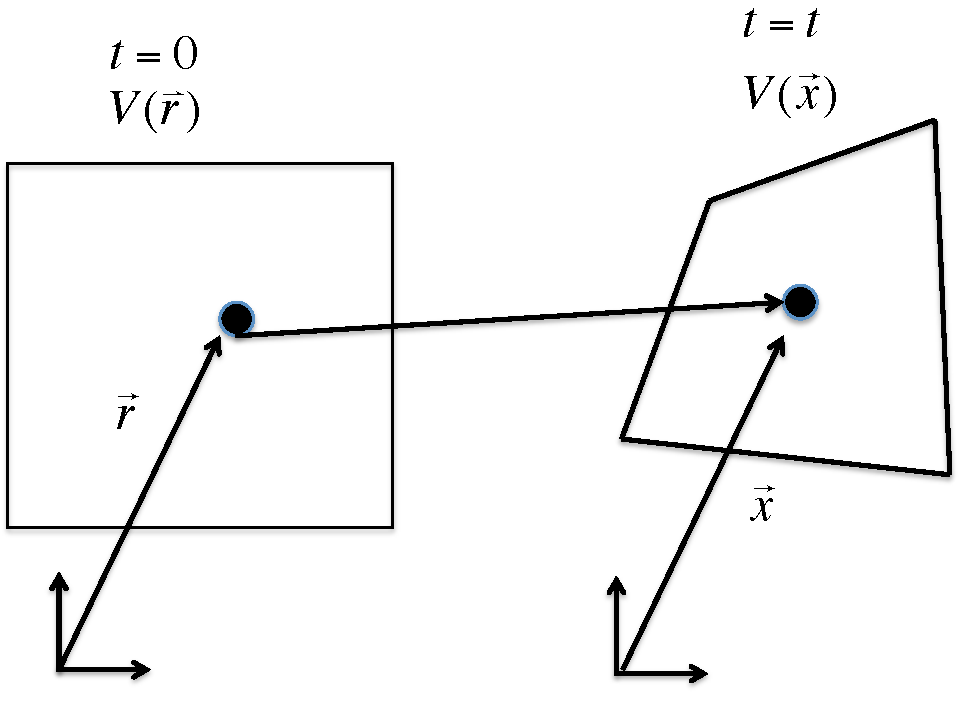
\includegraphics[width=8cm]{figure1.pdf}
\caption{Definition of the natural domain}
\label{fig:natural domain}
\end{figure} 

In \cref{eq:motion} we can understand $\vb{r}$ like a material (Lagrangian) variable and $\vb{X}$ like a spatial (or Eulerian) variable. Using the continuum mechanics analogy it is clear that the ``deformation'' process at the continuum level is fully characterized by the ``deformation'' gradient or Jacobian of the transformation \cref{eq:motion} and defined according to
\begin{equation}
\dd{X}_i=\pdv{X_i}{r_J}\dd{r}_J\equiv J_{iJ}\dd{r}_{J}
\label{eq:gradient}
\end{equation}
where $\dd{r}_{J}$ and $\dd{X}_i$ represent material vectors in the original and deformed configuration. From \cref{eq:gradient} it is evident that the Jacobian contains all the information describing the change of the physical sub-domain with respect to the natural element. For the element integration process we will assume that every element $V(\vb{r})$ in the natural domain deforms into the physical element $V_0(\vb{X})$, thus allowing us to write typical terms like the ones in the material stiffness matrix
\begin{equation}
\intL_{V(\vb{X})} \hat{B}_{ij}^K(\vb{X}) C_{ijkl} \hat{B}_{kl}^P(\vb{X}) dV(\vb{X})\equiv \intL_{V_0(\vb{r})} \hat{B}_{ij}^K(\vb{r}) C_{ijkl} \hat{B}_{kl}^P(\vb{r})J dV_0(\vb{r})
\label{eq:matmatrix}
\end{equation}
where we have used $dV(\vb{X})=JdV(\vb{r})$, with $J$ being the determinant of the deformation gradient and in general we transform functions between the natural and physical space making use of \cref{eq:motion} according to
\begin{equation}
f(\vb{r})=F[\vb{X}(\vb{r})]
\label{eq:funtrans}
\end{equation}


\subsubsection*{Interpolation scheme}
Having identified the fact that the integration process will take place in the natural domain, we will approach the interpolation process directly in this natural space. In the case of the displacement based finite element method all the involved variables will then be obtained via interpolation of nodal displacements. For instance, assume that a given problem variable is defined in the physical space by the tensor $\Phi_{ik...p}(\vb{X})$. The interpolated variable is then written like;

\begin{equation}
\Phi_{ij...p}(\vb{X})=H_{ij...p}^K(\vb{r})\hat{u}^K
\label{eq:interpol}
\end{equation}

where $\hat{u}^K$ represents a vector of nodal points displacements, see \cref{fig:interpol nat dom}, and $H_{ij...p}^K(\vb{r})$ is an interpolator which keeps the tensorial character of the original physical variable $\Phi_{ik...p}(\vb{X})$ and where the super-index makes reference to a nodal identifier (with the summation convention in place).


\begin{figure}[h]
\centering
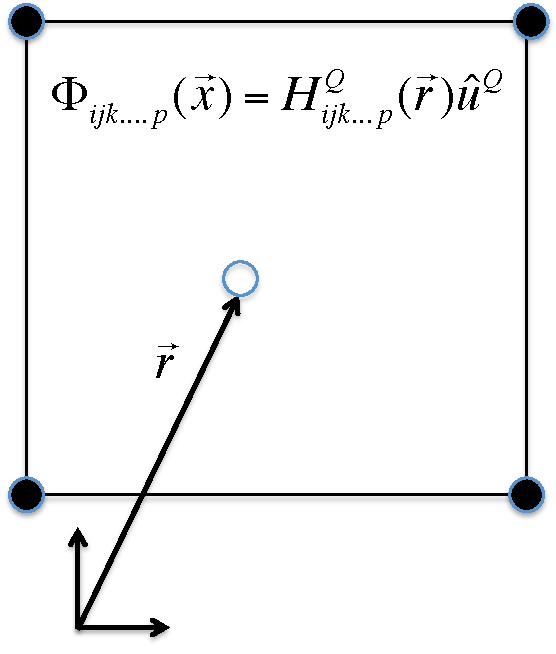
\includegraphics[width=4cm]{figure2.pdf}
\caption{General interpolation strategy in the natural domain}
\label{fig:interpol nat dom}
\end{figure}
 


Since the primary variable corresponds to displacements it must be kept in mind that $H_{ij...p}^K(\vb{r})$ corresponds to combinations of derivatives (or other arbitrary combinations) of the basic element shape functions defined in;


\begin{equation}
u_i(\vb{X})=N_i^K(\vb{r})\hat{u}^K
\label{eq:el interpol}
\end{equation}



For the general interpolation process we need two kinds of transformations.  First we need to transform integrals over the physical space into integrals into the natural space which corresponds to
\begin{equation}
\intL_{V(\vb{X})} F(\vb{X})dV(\vb{X})\equiv \intL_{V_0(\vb{r})} f(\vb{r})J dV_0(\vb{r})
\label{gen trans}
\end{equation}



Second we need to relate spatial differentiation in both, the physical and spatial domains.  Let us define these operators like $\nabla_i^X$ and $\nabla_I^r$ respectively. It then follows from \cref{eq:funtrans} that
\begin{equation}
\dfrac{\partial F}{\partial X_i}=\dfrac{\partial f}{\partial r_J}\dfrac{\partial r_J}{\partial X_i}
\label{eq:chain}
\end{equation}
from where we can establish the connection between the two operators like


\begin{equation}
\nabla_i^X=J_{iJ}^{-1}\nabla_J^r
\label{eq:fundamental}
\end{equation}


\subsubsection*{The fundamental interpolator}
We further define the fundamental interpolator giving rise to gradients of the primary displacement variable in the physical space according to
\begin{equation}
u_{i,j}(\vb{X})=L_{ij}^K(\vb{r})\hat{u}^K
\label{eq:fund operator}
\end{equation}


This fundamental interpolator  $L_{ik}^K(\vb{r})$ is derived after using \cref{eq:el interpol} and \cref{eq:fundamental} in the physical displacement gradient definition as shown next
\begin{align*}
u_{i,j}(\vb{X})&=\nabla_j^X u_i(\vb{X})\\
u_{i,j}(\vb{X})&=\nabla_j^X N_i^K(\vb{r})\hat{u}^K\\
u_{i,j}(\vb{X})&=J_{jQ}^{-1}\nabla_Q^r N_i^K(\vb{r})\hat{u}^K\\
u_{i,j}(\vb{X})&=J_{jQ}^{-1}N_{i,Q}^K(\vb{r})\hat{u}^K
\end{align*}
then
\begin{equation}
L_{ij}^K(\vb{r})=J_{jQ}^{-1}N_{i,Q}^K(\vb{r})
\label{eq:fundamental interpolator}
\end{equation}

\subsubsection*{Elemental stiffness matrix}
The elemental material stiffness matrix computed in the natural domain of \cref{fig:Nat domain} reads

\begin{equation}
K^{KP}=\intL_{V_0(\vb{r})} \hat{B}_{ij}^K(\vb{r}) C_{ijkl} \hat{B}_{kl}^P(\vb{r})J dV_0(\vb{r})\equiv \intL_{r=-1}^{r=+1}\intL_{s=-1}^{s=+1} \hat{B}_{ij}^K(r,s) C_{ijkl} \hat{B}_{kl}^P(r,s)J(r,s) \mathrm{d}r\mathrm{d}s
\label{eq:elematrix}
\end{equation}



\begin{figure}[h]
\centering
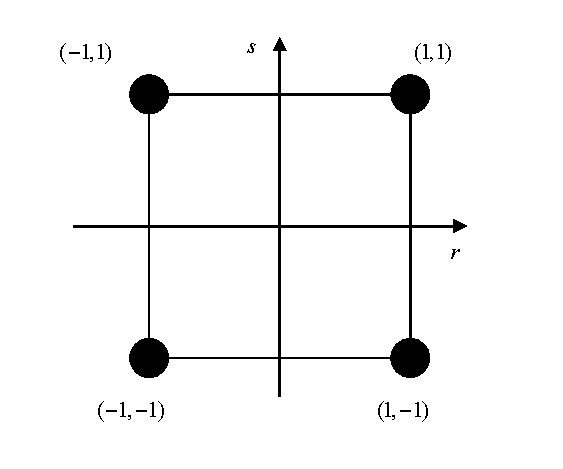
\includegraphics[width=6cm]{figure3.pdf}
\caption{Natural domain of integration}
\label{fig:Nat domain}
\end{figure}
 

Once the interpolator $\hat{B}_{ij}^K(\vb{r})$ has been identified the elemental stiffness matrix is obtained via numerical integration (quadrature) as described in \eqref{eq:eleintegration}

\begin{equation}
\intL_{r=-1}^{r=+1}\intL_{s=-1}^{s=+1} \hat{B}_{ij}^K(r,s) C_{ijkl} \hat{B}_{kl}^P(r,s)J(r,s) \mathrm{d}r\mathrm{d}s\approx \sum_{i,j=1}^\text{NGPTS} \alpha_i \alpha_j \hat{B}_{kl}^K(r_i,s_j)C_{ijkl} \hat{B}_{kl}^P(r_i,s_j) J(r_i,s_j)
\label{eq:eleintegration}
\end{equation}


and where NGPTS corresponds to the number of integration points, $\alpha_j$ is a weighting factor and $r_i,s_j$   are the coordinates of a typical point $\vb{r}$ in the natural space of \cref{fig:Nat domain}.

 
\begin{figure}[h]
\centering
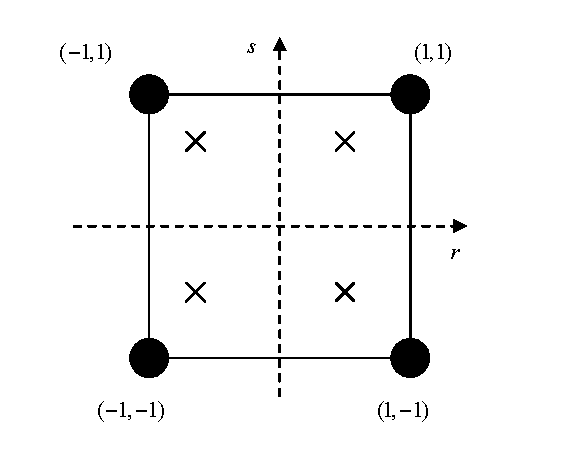
\includegraphics[width=6cm]{figure4.pdf}
\caption{Natural integration domain showing quadrature evaluation nodes}
\label{fig:integration domain}
\end{figure}	 


One important aspect of the numerical integration that has to be kept in mind is accuracy.  Depending on the particularly selected integration scheme, the number of introduced integration points fixes the maximum polynomial order of the considered functions that can be integrated accurately.  In the case of the integrand in \cref{eq:eleintegration}, it is clear that this order increases as the distortion of the physical element  with respect to the natural element increases.  One way of dealing with this dependency of accuracy with element distortion is to make use of adaptative integration techniques which are numerically expensive.  What is actually done in standard FEM analysis is to choose the number of quadrature points beforehand and introduce distortion related error criteria inside the code in such a way that some sort of validation is performed before the numerical integration process is started.

\subsubsection*{Strain displacement interpolator for the infinitesimal strain tensor}
The $Q$-th nodal contribution to the infinitesimal strain-displacement interpolator can be obtained in explicit form as follows. Let $L_x^Q$ and $L_y^Q$ be the spatial differential operators in $x$ and $y$ respectively. We have after expanding \cref{eq:fundamental interpolator}
%
\begin{align*}
L_x^Q & = J_{xP}^{-1}\frac{\partial N^Q}{\partial r_P} \equiv J_{xr}^{-1}\frac{\partial N^Q}{\partial r} + J_{xs}^{-1}\frac{\partial N^Q}{\partial s}\\
L_y^Q & = J_{yP}^{-1}\frac{\partial N^Q}{\partial r_P} \equiv J_{yr}^{-1}\frac{\partial N^Q}{\partial r} + J_{ys}^{-1}\frac{\partial N^Q}{\partial s}
\end{align*}
%
or in matrix form
%
\begin{equation}
\begin{Bmatrix}
L_x^Q\\
L_y^Q
\end{Bmatrix} = 
\begin{bmatrix}
J_{xP}^{-1} &J_{xs}^{- 1}\\
J_{yr}^{-1} &J_{ys}^{- 1}
\end{bmatrix}
\begin{Bmatrix}
\frac{\partial N^Q}{\partial r}\\
\frac{\partial N^Q}{\partial s}
\end{Bmatrix}
\end{equation}

The $Q$-th nodal contribution is then assembled as follows;


\begin{equation}
\begin{Bmatrix}
\pdv{u}{x}\\
\pdv{v}{y}\\
\pdv{u}{y} + \pdv{v}{x}
\end{Bmatrix} =
\begin{bmatrix}
 &L_x^Q &0 \\
\cdots &0 &L_y^Q &\cdots\\
 &L_y^Q &L_{xy}^Q
\end{bmatrix}
\begin{Bmatrix}
\vdots\\
u^Q\\
v^Q\\
\vdots
\end{Bmatrix}
\label{eq:strain inter}
\end{equation}

\begin{algorithm}[H]
    \SetAlgoLined
    \KwData{Nodal coordinates $x^Q$}
    \KwResult{Strain-displacement interpolator $B_{ij}^Q$ }
    Compute Jacobian ${J_{iJ}} = \pdv{N_i^Q}{r_J}{\hat x}^Q$\\
    Invert Jacobian  ${J_{iJ}} \to J_{iJ}^{ - 1}$\\
    Compute fundamental interpolator $L_{ij}^Q = J_{jP}^{ - 1}\pdv{N_i^Q}{r_P}$\\
    Assemble $B_{ij}^Q = \frac{1}{2}\left( {L_{ij}^Q + L_{ji}^Q} \right)$ 
    \caption{Strain-displacement interpolator}
\end{algorithm}
\newpage
\subsection*{Problems}



